%Please use LuaLaTeX or XeLaTeX
\documentclass[11pt,aspectratio=169]{beamer}

\title{Operating the Mu3e SciFi Detector: Control, Monitoring and Calibration}
\date[Mu3e]{S3P3 Final Event, Bern\\September 4th, 2026}
\author{Giacomo Moretti \\ \small Supervisor: Marius K\"oppel}
\institute[D-PHYS, ETH Z\"urich]{D-PHYS Institute for Particle Physics and Astrophysics}

\usetheme{eth}
\usetikzlibrary{positioning, arrows.meta, calc, shapes.geometric, backgrounds, fit, decorations.pathmorphing}

\usepackage{fontspec}
\setsansfont{Avenir Next}[UprightFont=* Medium, BoldFont=* Demi Bold, ItalicFont=* Medium Italic]

\colorlet{titlefgcolor}{ETHBlue}
\colorlet{accentcolor}{ETHRed}

% ------------------------------------------------------------------
% Pillar color coding -- used consistently across every diagram
% ------------------------------------------------------------------
\definecolor{instcolor}{RGB}{198,110,0}    % Installation -- orange
\colorlet{uicolor}{ETHBlue}                % User Interface -- blue
\colorlet{pwrcolor}{ETHPetrol}             % Power -- teal
\colorlet{calcolor}{ETHRed}                % Calibration -- red
\definecolor{savecolor}{RGB}{60,135,40}    % Saving -- green
\colorlet{confcolor}{ETHPurple}            % Configuration -- magenta
\definecolor{metacolor}{RGB}{72,78,96}     % Big picture / wrap-up -- slate

% ------------------------------------------------------------------
% Reusable tikz styles
% ------------------------------------------------------------------
\tikzset{
  boxhw/.style   ={draw=ETHGray,   thick, rounded corners, fill=ETHGray!10,   minimum height=1cm, minimum width=2.3cm, align=center, font=\small},
  boxinst/.style ={draw=instcolor, thick, rounded corners, fill=instcolor!20, minimum height=1cm, minimum width=2.3cm, align=center, font=\small},
  boxui/.style   ={draw=uicolor,   thick, rounded corners, fill=uicolor!18,   minimum height=1cm, minimum width=2.3cm, align=center, font=\small},
  boxpwr/.style  ={draw=pwrcolor,  thick, rounded corners, fill=pwrcolor!20,  minimum height=1cm, minimum width=2.3cm, align=center, font=\small},
  boxcal/.style  ={draw=calcolor,  thick, rounded corners, fill=calcolor!18,  minimum height=1cm, minimum width=2.3cm, align=center, font=\small},
  boxsave/.style ={draw=savecolor, thick, rounded corners, fill=savecolor!20, minimum height=1cm, minimum width=2.3cm, align=center, font=\small},
  boxconf/.style ={draw=confcolor, thick, rounded corners, fill=confcolor!18, minimum height=1cm, minimum width=2.3cm, align=center, font=\small},
  boxmeta/.style ={draw=metacolor, thick, rounded corners, fill=metacolor!18, minimum height=1cm, minimum width=2.3cm, align=center, font=\small},
  boxblue/.style ={draw=ETHBlue,   thick, rounded corners, fill=ETHBlue!10,   minimum height=1cm, minimum width=2.3cm, align=center, font=\small},
  boxred/.style  ={draw=ETHRed,    thick, rounded corners, fill=ETHRed!10,    minimum height=1cm, minimum width=2.3cm, align=center, font=\small},
  arr/.style     ={-{Stealth[length=2.2mm]}, thick, draw=ETHGray},
  arrthin/.style ={-{Stealth[length=1.8mm]}, draw=ETHGray!70},
  commit/.style  ={circle, draw=ETHBlue, fill=ETHBlue, minimum size=2.2mm, inner sep=0pt},
  dotinst/.style ={circle, draw=instcolor, fill=instcolor, minimum size=2.4mm, inner sep=0pt},
  dotcal/.style  ={circle, draw=calcolor,  fill=calcolor,  minimum size=2.4mm, inner sep=0pt},
}

% ------------------------------------------------------------------
% Status pill: \statuspill{color}{\faIcon}{text}
% ------------------------------------------------------------------
\newcommand{\statuspill}[3]{%
  \tikz[baseline=-0.65ex]{\node[rounded corners=2pt, inner sep=3pt, fill=#1!12, draw=#1, thick, font=\scriptsize\bfseries, text=#1!55!black]{#2~#3};}%
}

% ------------------------------------------------------------------
% Section divider: \dividerframe{color}{floor index 0-7, or -1}{Title text}
% Draws a mini, unlabelled copy of the building diagram on the right --
% every floor already passed is filled in with its own gradient color
% (like a battery charging), the current floor is bold, the rest stay faded.
% ------------------------------------------------------------------
\newcommand{\dividerframe}[3]{%
  {\setbeamertemplate{footline}{}
  \begin{frame}[plain,noframenumbering]
    \begin{tikzpicture}[remember picture, overlay]
      \fill[white] (current page.south west) rectangle (current page.north east);
      \fill[#1] (current page.south west) rectangle ([xshift=3.2mm]current page.north west);
      \node[black!80, font=\fontsize{30}{30}\selectfont, anchor=west] at ([xshift=20mm]current page.west) {#3};
      \draw[#1, line width=0.8pt] ([xshift=20mm,yshift=-9mm]current page.west) -- ([xshift=95mm,yshift=-9mm]current page.west);
      \begin{scope}[shift={($(current page.east)+(-32mm,0)$)}]
        \foreach \i/\fc/\dc in {0/ETHGray!28/ETHGray,
                                 1/ETHGray!72!ETHBlue!32/ETHGray!72!ETHBlue,
                                 2/ETHGray!52!ETHBlue!32/ETHGray!52!ETHBlue,
                                 3/ETHGray!37!ETHBlue!32/ETHGray!37!ETHBlue,
                                 4/ETHGray!25!ETHBlue!32/ETHGray!25!ETHBlue,
                                 5/ETHGray!16!ETHBlue!32/ETHGray!16!ETHBlue,
                                 6/ETHGray!8!ETHBlue!32/ETHGray!8!ETHBlue,
                                 7/ETHBlue!28/ETHBlue} {
          \ifnum\i=#2
            \node[rounded corners, minimum width=1.5cm, minimum height=0.4cm, fill=#1, draw=#1] at (0,{\i*0.5cm-1.75cm}) {};
          \else
            \ifnum\i<#2
              \node[rounded corners, minimum width=1.5cm, minimum height=0.4cm, fill=\fc, draw=\dc] at (0,{\i*0.5cm-1.75cm}) {};
            \else
              \node[rounded corners, minimum width=1.5cm, minimum height=0.4cm, fill=ETHGray!10, draw=ETHGray!30] at (0,{\i*0.5cm-1.75cm}) {};
            \fi
          \fi
        }
      \end{scope}
    \end{tikzpicture}
  \end{frame}}%
}

% ------------------------------------------------------------------
% Opening thesis: a closed loop of organs, not a linear roadmap.
% ------------------------------------------------------------------
\newcommand{\roadmapframe}{%
\begin{frame}{How it all fits together}
  \begin{columns}[onlytextwidth,c]
    \begin{column}{0.42\textwidth}
      \begin{center}
      \resizebox{\linewidth}{!}{%
      \begin{tikzpicture}[every node/.style={align=center, rounded corners, thick,
            minimum width=2.3cm, minimum height=1.05cm, font=\small}]
        \node[fill=instcolor!22, draw=instcolor, text=instcolor]  (hw)   at (90:1.85cm)  {Detector};
        \node[fill=metacolor!22, draw=metacolor, text=metacolor]  (py)   at (0:1.85cm)   {Python\\scripts};
        \node[fill=savecolor!22, draw=savecolor, text=savecolor]  (odb)  at (-90:1.85cm) {Database};
        \node[fill=uicolor!22,   draw=uicolor,   text=uicolor]    (page) at (180:1.85cm) {Custom\\page};
        \draw[-{Stealth[length=3mm]}, thick, ETHGray!55] (hw)   to[bend left=18] (py);
        \draw[-{Stealth[length=3mm]}, thick, ETHGray!55] (py)   to[bend left=18] (odb);
        \draw[-{Stealth[length=3mm]}, thick, ETHGray!55] (odb)  to[bend left=18] (page);
        \draw[-{Stealth[length=3mm]}, thick, ETHGray!55] (page) to[bend left=18] (hw);
      \end{tikzpicture}%
      }
      \end{center}
    \end{column}
    \begin{column}{0.54\textwidth}
      \begin{itemize}\small\setlength{\itemsep}{4pt}
        \item \textbf{\textcolor{instcolor}{Detector}} -- matters once a script can drive it.
        \item \textbf{\textcolor{metacolor}{Python scripts}} -- matter once the result is saved.
        \item \textbf{\textcolor{savecolor}{Database}} -- matters once the page shows it back.
        \item \textbf{\textcolor{uicolor}{Custom page}} -- matters once a shifter can act on it.
      \end{itemize}
    \end{column}
  \end{columns}
  \medskip
  \small This is a control and monitoring system: no single piece works alone. Every step in this loop matters equally.
\end{frame}
}

% ------------------------------------------------------------------
% Image placeholder: \imgph{width}{height}{description}
% ------------------------------------------------------------------
\newcommand{\imgph}[3]{%
  \begin{tikzpicture}
    \node[draw=ETHGray, dashed, ultra thick, minimum width=#1, minimum height=#2,
          fill=ETHGray!6, align=center, font=\small\itshape, text=ETHGray!70!black,
          inner sep=3mm]{\faImage\\[2mm]#3};
  \end{tikzpicture}%
}

\begin{document}

\def\titlefigure{}
\setlength{\titleboxwidth}{0.85\textwidth}
\titleframe

% ==================================================================
\begin{frame}{Why search for $\mu \to eee$ -- and why it is hard}
  \vspace{-5mm}
  \begin{columns}[onlytextwidth,T]
    \begin{column}{0.2\textwidth}
      \vspace{3mm}
      {\centering\small\textbf{\textcolor{metacolor}{Why search}}\par}
      \smallskip
      \tiny
      \begin{itemize}\setlength{\itemsep}{2pt}
        \item \textcolor{metacolor}{Charged-lepton flavour violation}: \textbf{never observed}.
        \item $\mu^+\!\to\! e^+e^-e^+$ is one of the \textbf{\textcolor{metacolor}{``golden'' channels}}.
        \item Yet flavour \textbf{is} violated for neutrinos: \textcolor{metacolor}{$\nu_\mu\!\to\!\nu_e$}.
      \end{itemize}
    \end{column}
    \begin{column}{0.6\textwidth}\centering
      \vspace{2mm}
      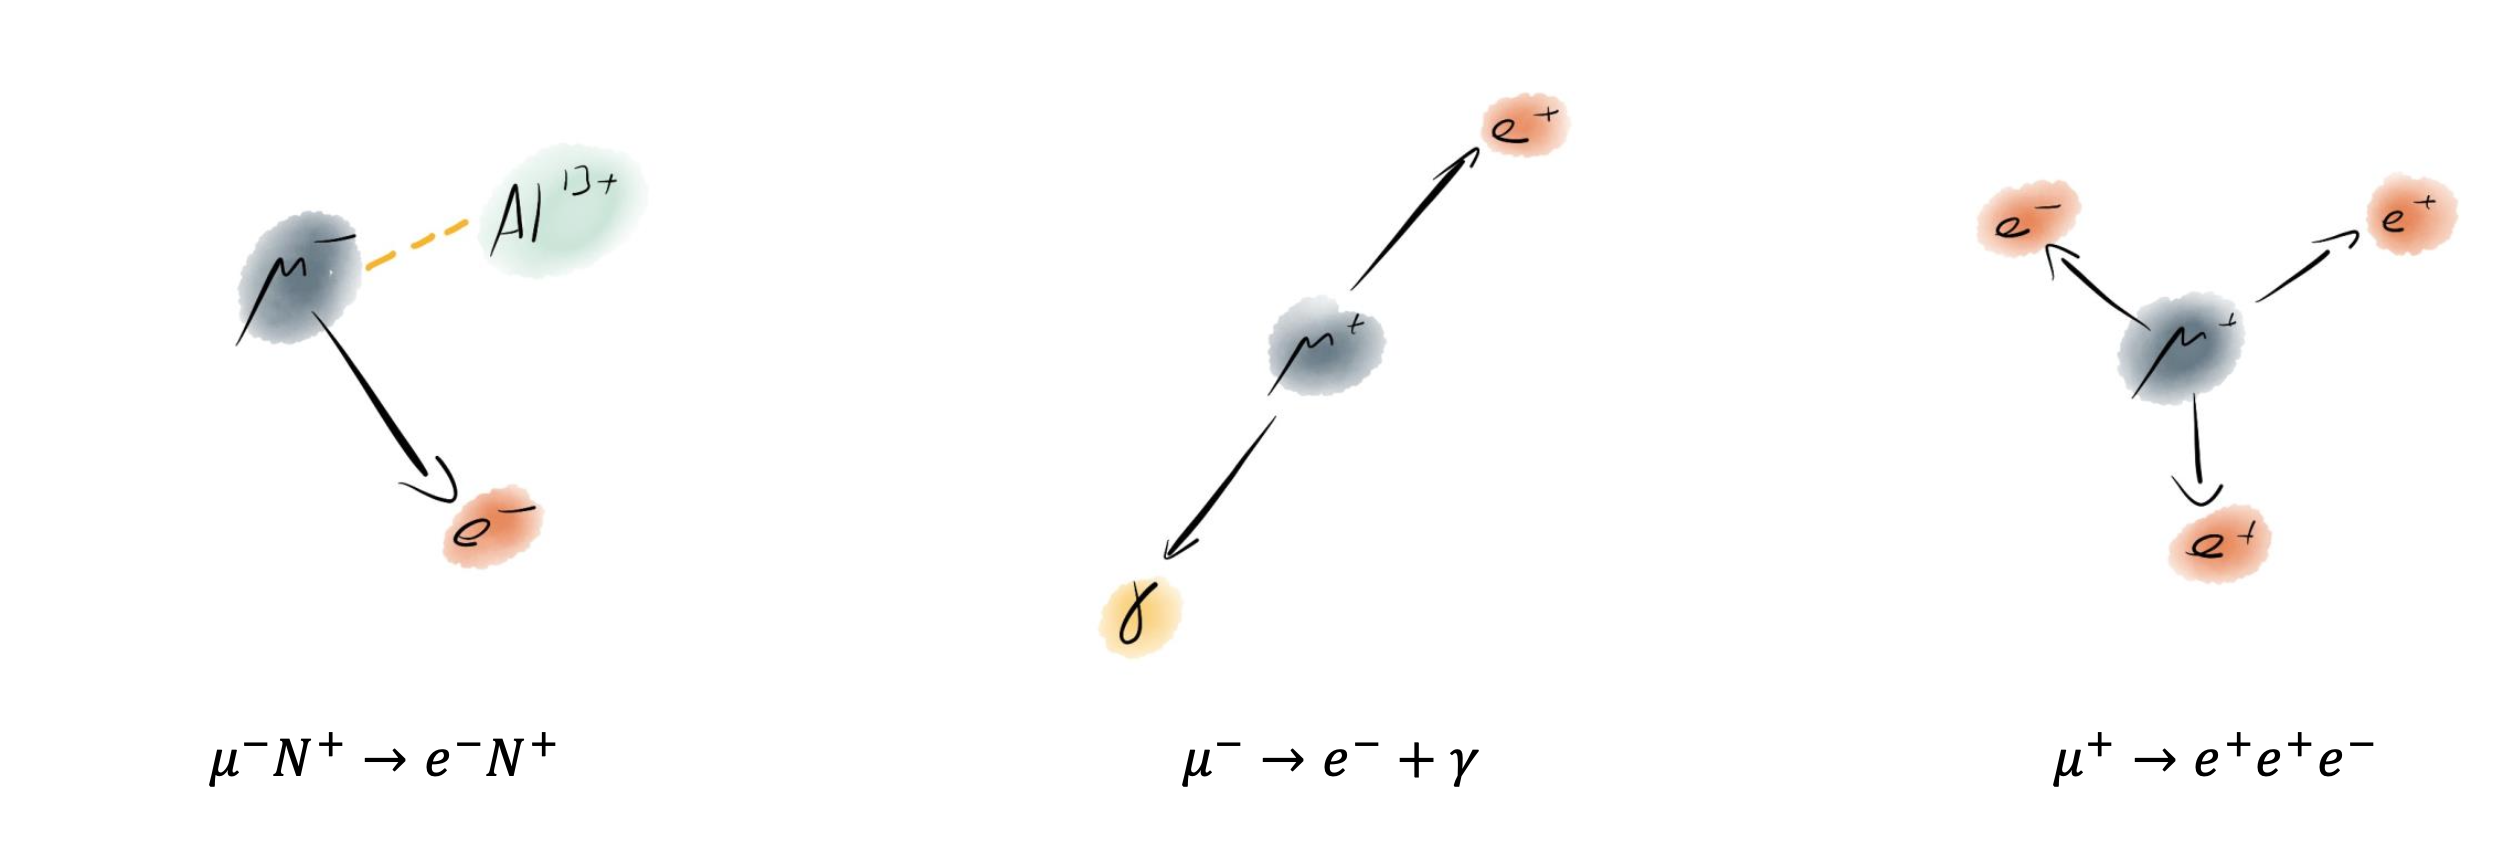
\includegraphics[width=0.78\linewidth]{../imgs/golden_channels.png}\\[0.5mm]
      \begin{minipage}[c]{0.45\linewidth}\centering
        
\includegraphics[width=\linewidth]{../imgs/nu_violation.png}
      \end{minipage}\hspace{2mm}%
      \begin{minipage}[c]{0.32\linewidth}\centering
        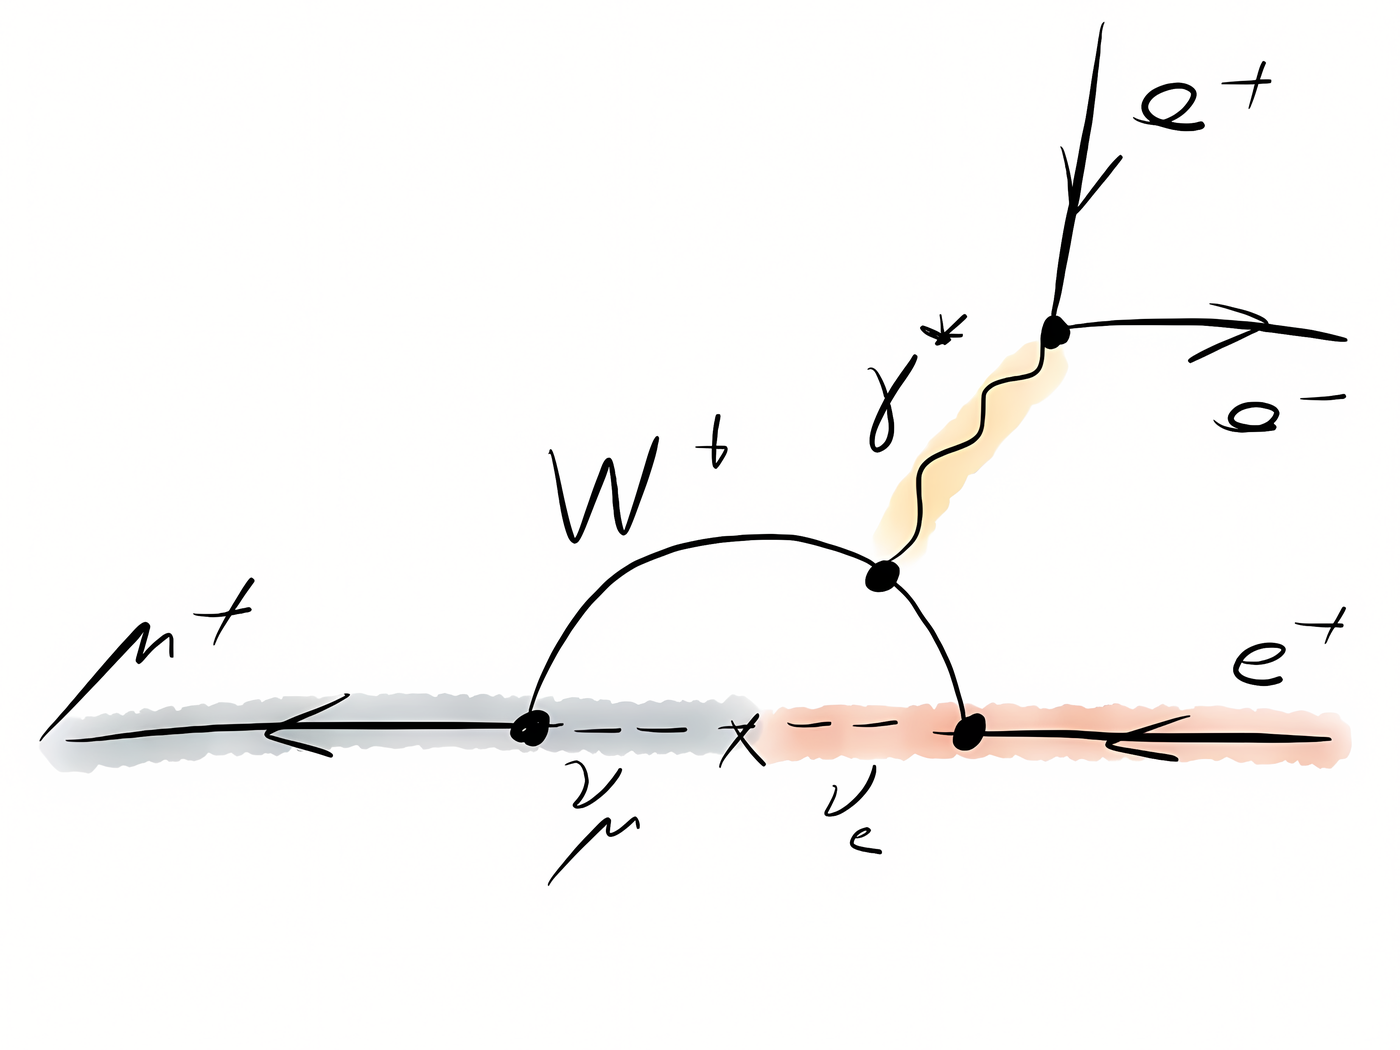
\includegraphics[width=\linewidth]{../imgs/mu3e_neutrino_osc.png}
      \end{minipage}\\[2mm]
      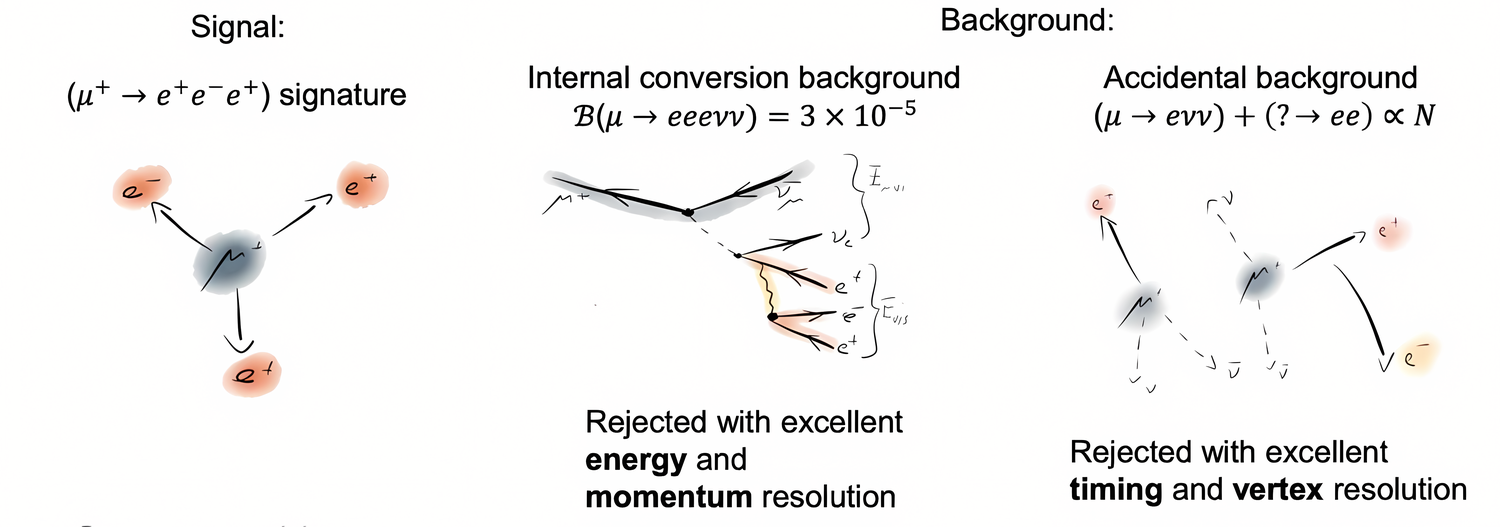
\includegraphics[width=\linewidth]{../imgs/signal_vs_bkg.png}
    \end{column}
    \begin{column}{0.2\textwidth}
      \vspace{3mm}
      {\centering\small\textbf{\textcolor{calcolor}{Why it is hard}}\par}
      \smallskip
      \tiny
      \begin{itemize}\setlength{\itemsep}{2pt}
        \item Continuous \textcolor{calcolor}{$10^8\,\mu$/s} beam.
        \item \textcolor{calcolor}{Internal conversion} $\mu\!\to\! eee\nu\nu$: beat with \textbf{\textcolor{uicolor}{energy}} $+$ \textbf{\textcolor{uicolor}{momentum}} resolution.
        \item \textcolor{calcolor}{Accidental combinations} $\propto$ rate: beat with \textbf{\textcolor{uicolor}{timing}} $+$ \textbf{\textcolor{uicolor}{vertex}} resolution.
      \end{itemize}
    \end{column}
  \end{columns}
\end{frame}

% ==================================================================
{
\setbeamertemplate{background}{%
  \begin{tikzpicture}
    \useasboundingbox (0,0) rectangle(\the\paperwidth,\the\paperheight);
    % --- images, as a backdrop ---
    \node[inner sep=0] at ([xshift=2mm, yshift=21mm]current page.center)
      {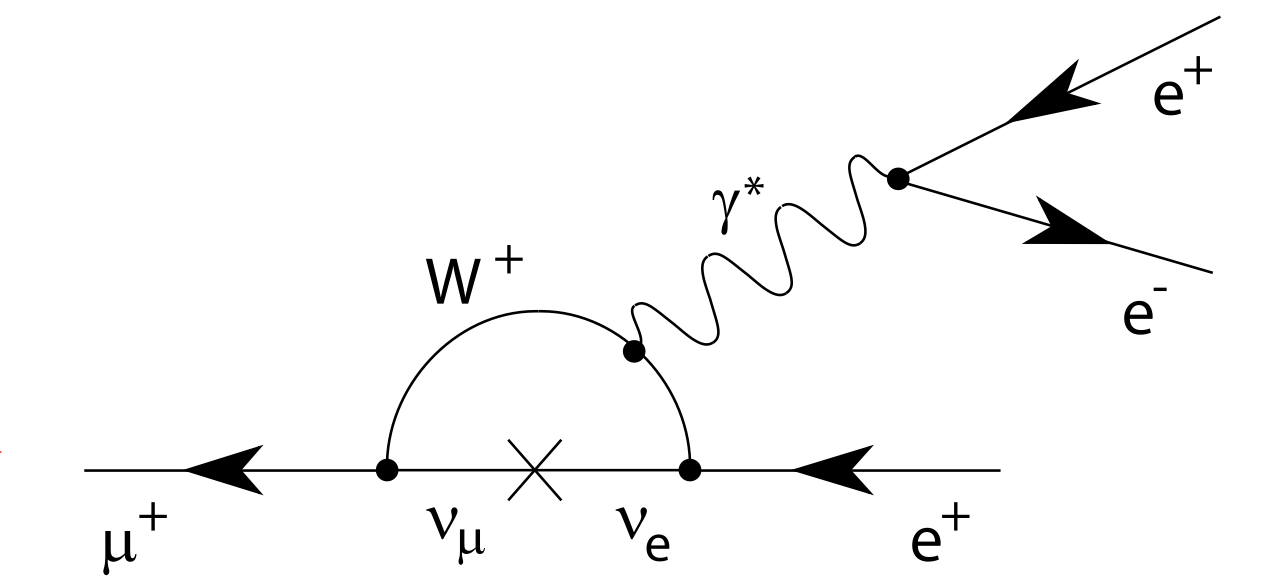
\includegraphics[width=43mm]{../imgs/penguin_diagram.png}};
    \node[inner sep=0] at ([xshift=53mm, yshift=21mm]current page.center)
      {\begin{minipage}{42mm}\centering
        
\includegraphics[width=\linewidth]{../imgs/mu3e_br.png}\\[2mm]
        
\includegraphics[width=\linewidth]{../imgs/SIDRUM_BR.png}
      \end{minipage}};
    \node[anchor=south west, inner sep=0] at ([xshift=8mm, yshift=12mm]current page.south west)
      {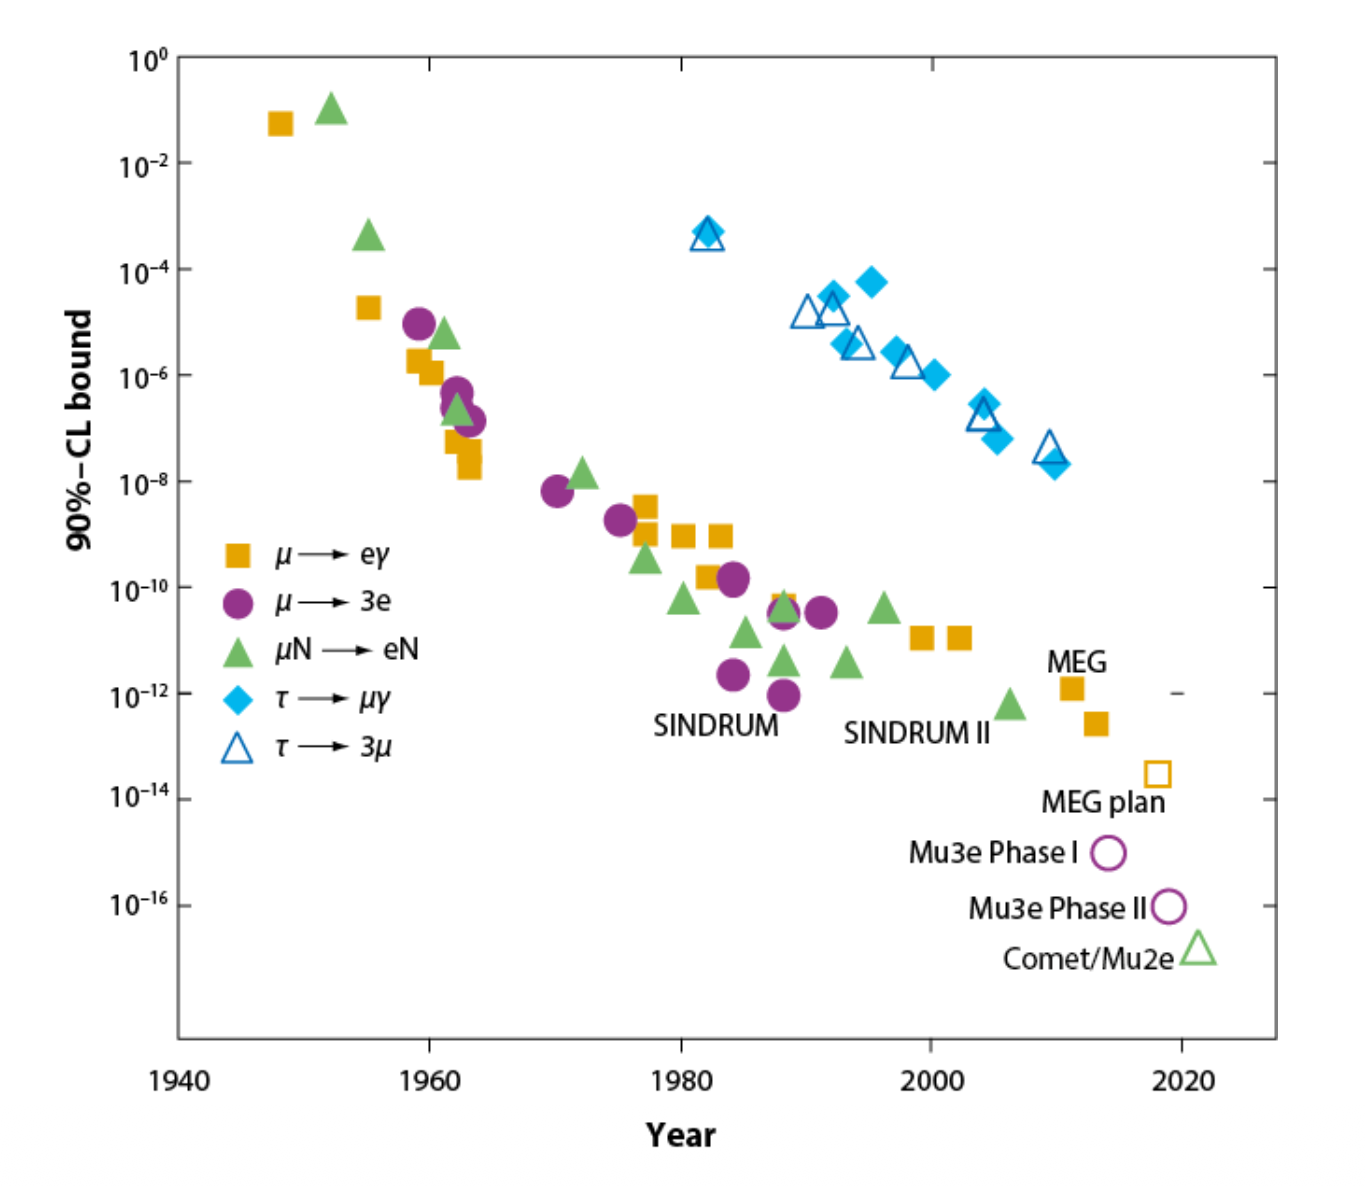
\includegraphics[width=42mm]{../imgs/CL_year.png}};
    \node[anchor=south east, inner sep=0] at ([xshift=-6mm, yshift=11mm]current page.south east)
      {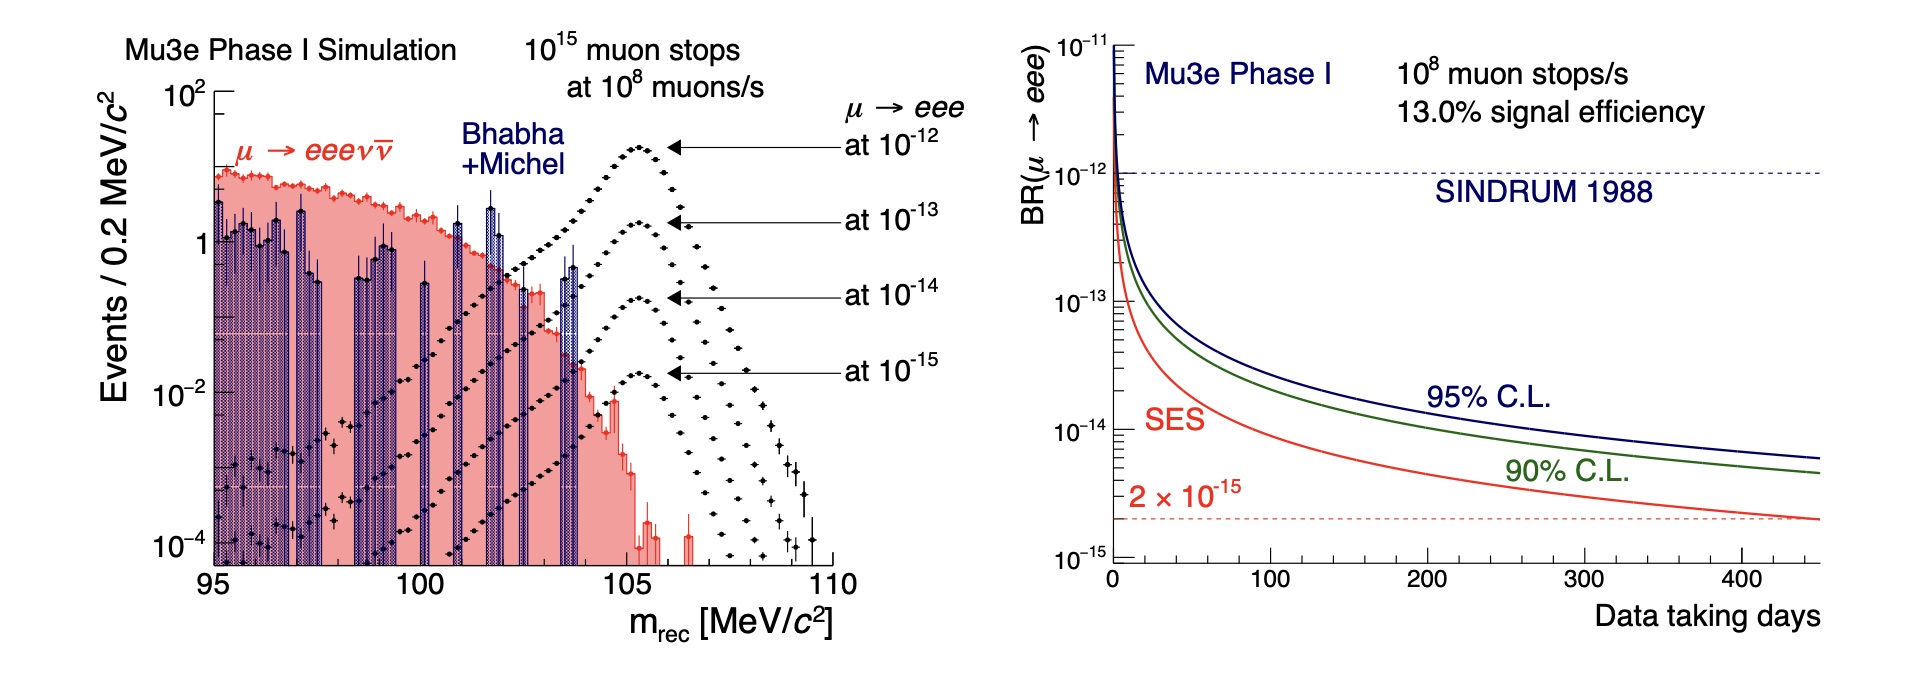
\includegraphics[width=104mm]{../imgs/physic_process_meas.png}};
    % --- overlaid text box (slide-4 style) ---
    \node[anchor=north west, align=left, font=\scriptsize,
          fill=white, fill opacity=0.9, text opacity=1, rounded corners,
          inner sep=7pt, text width=5.3cm]
      at ([xshift=3mm, yshift=-10mm]current page.north west) {%
        \hyphenpenalty=10000\exhyphenpenalty=10000
        \begin{itemize}\setlength{\itemsep}{3pt}\scriptsize
          \item SM: $\mu\to eee$ only via a \textcolor{metacolor}{$\nu$ loop} $\Rightarrow$
            $\text{BR}\sim10^{-54}$, \textcolor{savecolor}{background-free}.
          \item Any signal $=$ \textbf{\textcolor{savecolor}{unambiguous new physics}}.
          \item \textbf{\textcolor{metacolor}{SINDRUM}} $<10^{-12}$
            $\to$ \textcolor{uicolor}{Mu3e $10^{-16}$}: \textbf{\textcolor{calcolor}{four orders of magnitude}}.
        \end{itemize}};
  \end{tikzpicture}%
}
\begin{frame}{Four orders of magnitude}
\end{frame}
}

% ==================================================================
\begin{frame}{Experimental strategy}
  \begin{center}
  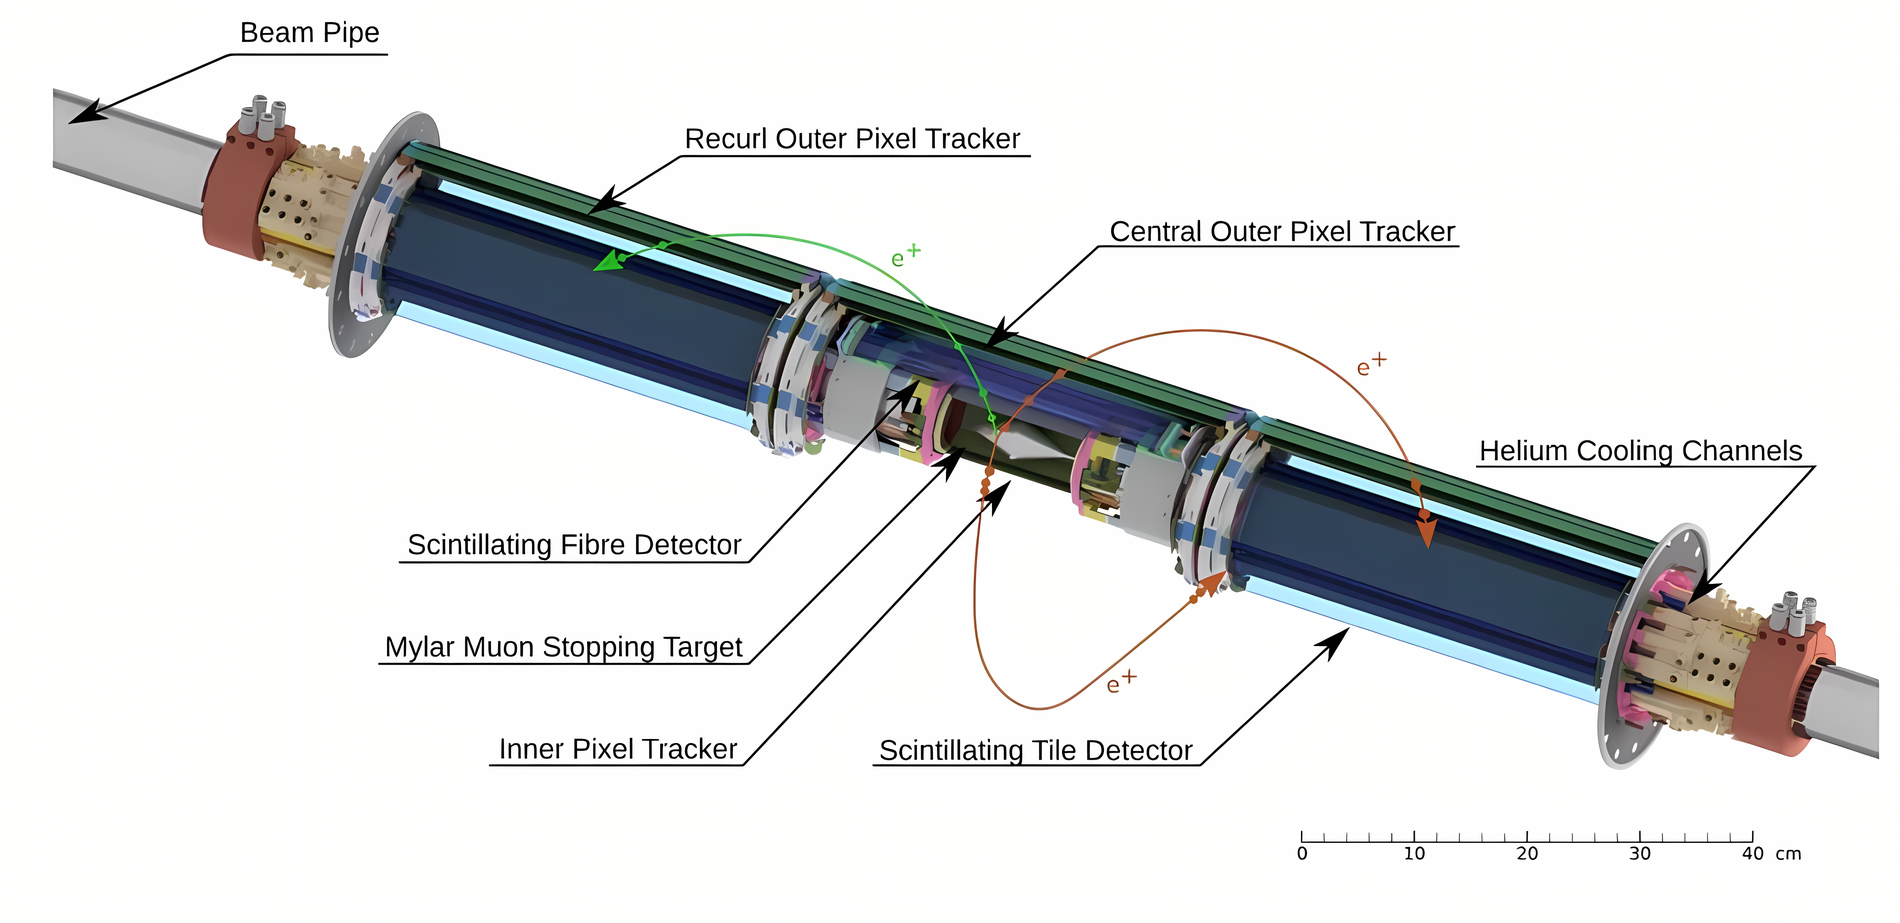
\includegraphics[width=\linewidth]{../imgs/detector_render_details.png}
  \end{center}
\end{frame}

% ==================================================================
{
\setbeamertemplate{background}{%
  \begin{tikzpicture}
    \useasboundingbox (0,0) rectangle(\the\paperwidth,\the\paperheight);
    \node[anchor=north, inner sep=0] (img) at ([yshift=-10mm]current page.north)
      {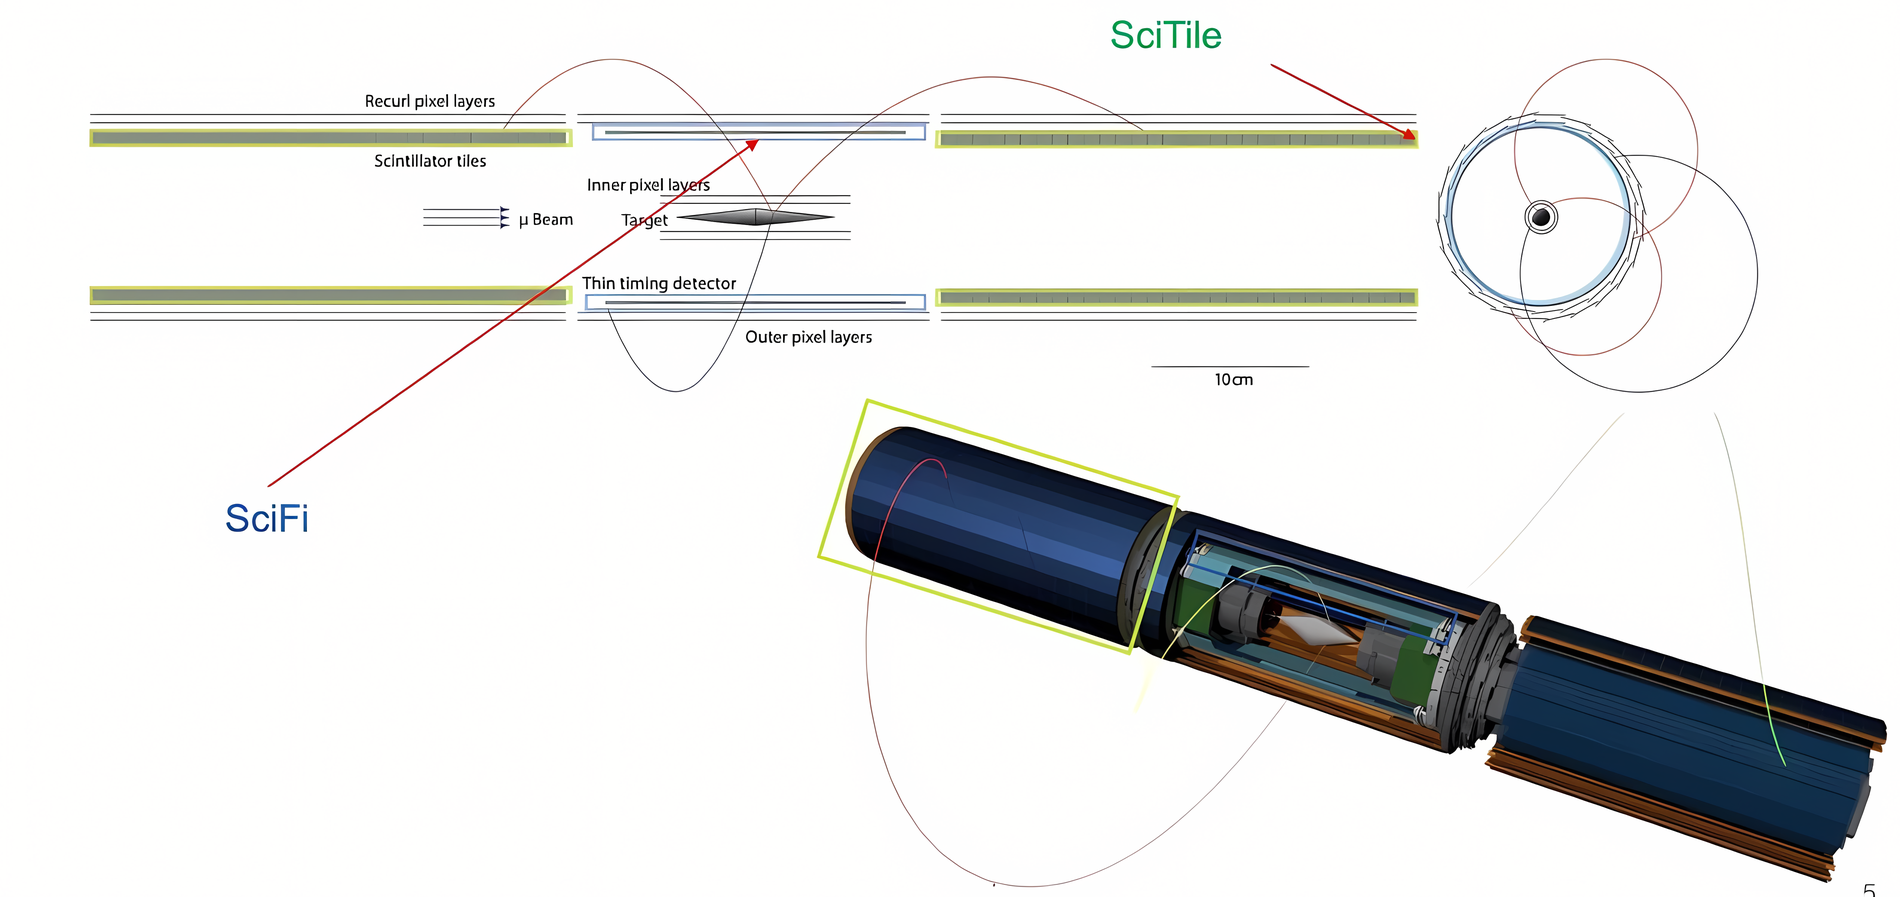
\includegraphics[width=\the\paperwidth-14mm]{../imgs/time_layer.png}};
    \node[anchor=north west, align=left, font=\footnotesize,
          fill=white, fill opacity=0.88, text opacity=1, rounded corners,
          inner sep=7pt]
      at ([xshift=4mm, yshift=22mm]img.south west) {%
        \hyphenpenalty=10000\exhyphenpenalty=10000
        \begin{minipage}[t]{3.8cm}\raggedright
          \textbf{\textcolor{metacolor}{Goals}}\\[2pt]
          \textcolor{uicolor}{time coincidence}, \textcolor{calcolor}{charge identification}, and \textcolor{savecolor}{global event reconstruction}.
        \end{minipage}\hspace{4mm}%
        \begin{minipage}[t]{3.4cm}\raggedright
          \textbf{\textcolor{metacolor}{Timing resolution}}
          \begin{itemize}\setlength{\itemsep}{1pt}\setlength{\topsep}{1pt}\footnotesize
            \item \textbf{\textcolor{pwrcolor}{SciFi}} $<200\,$ps
            \item \textbf{\textcolor{savecolor}{SciTile}} $<50\,$ps
            \item \textbf{\textcolor{calcolor}{Pixel}} $<26\,$ns
          \end{itemize}
        \end{minipage}};
  \end{tikzpicture}%
}
\begin{frame}{Timing layers in Mu3e}
\end{frame}
}

% ==================================================================
{
\setbeamertemplate{background}{%
  \begin{tikzpicture}
    \useasboundingbox (0,0) rectangle(\the\paperwidth,\the\paperheight);
    \node[anchor=north] at ([yshift=-1mm]current page.north)
      {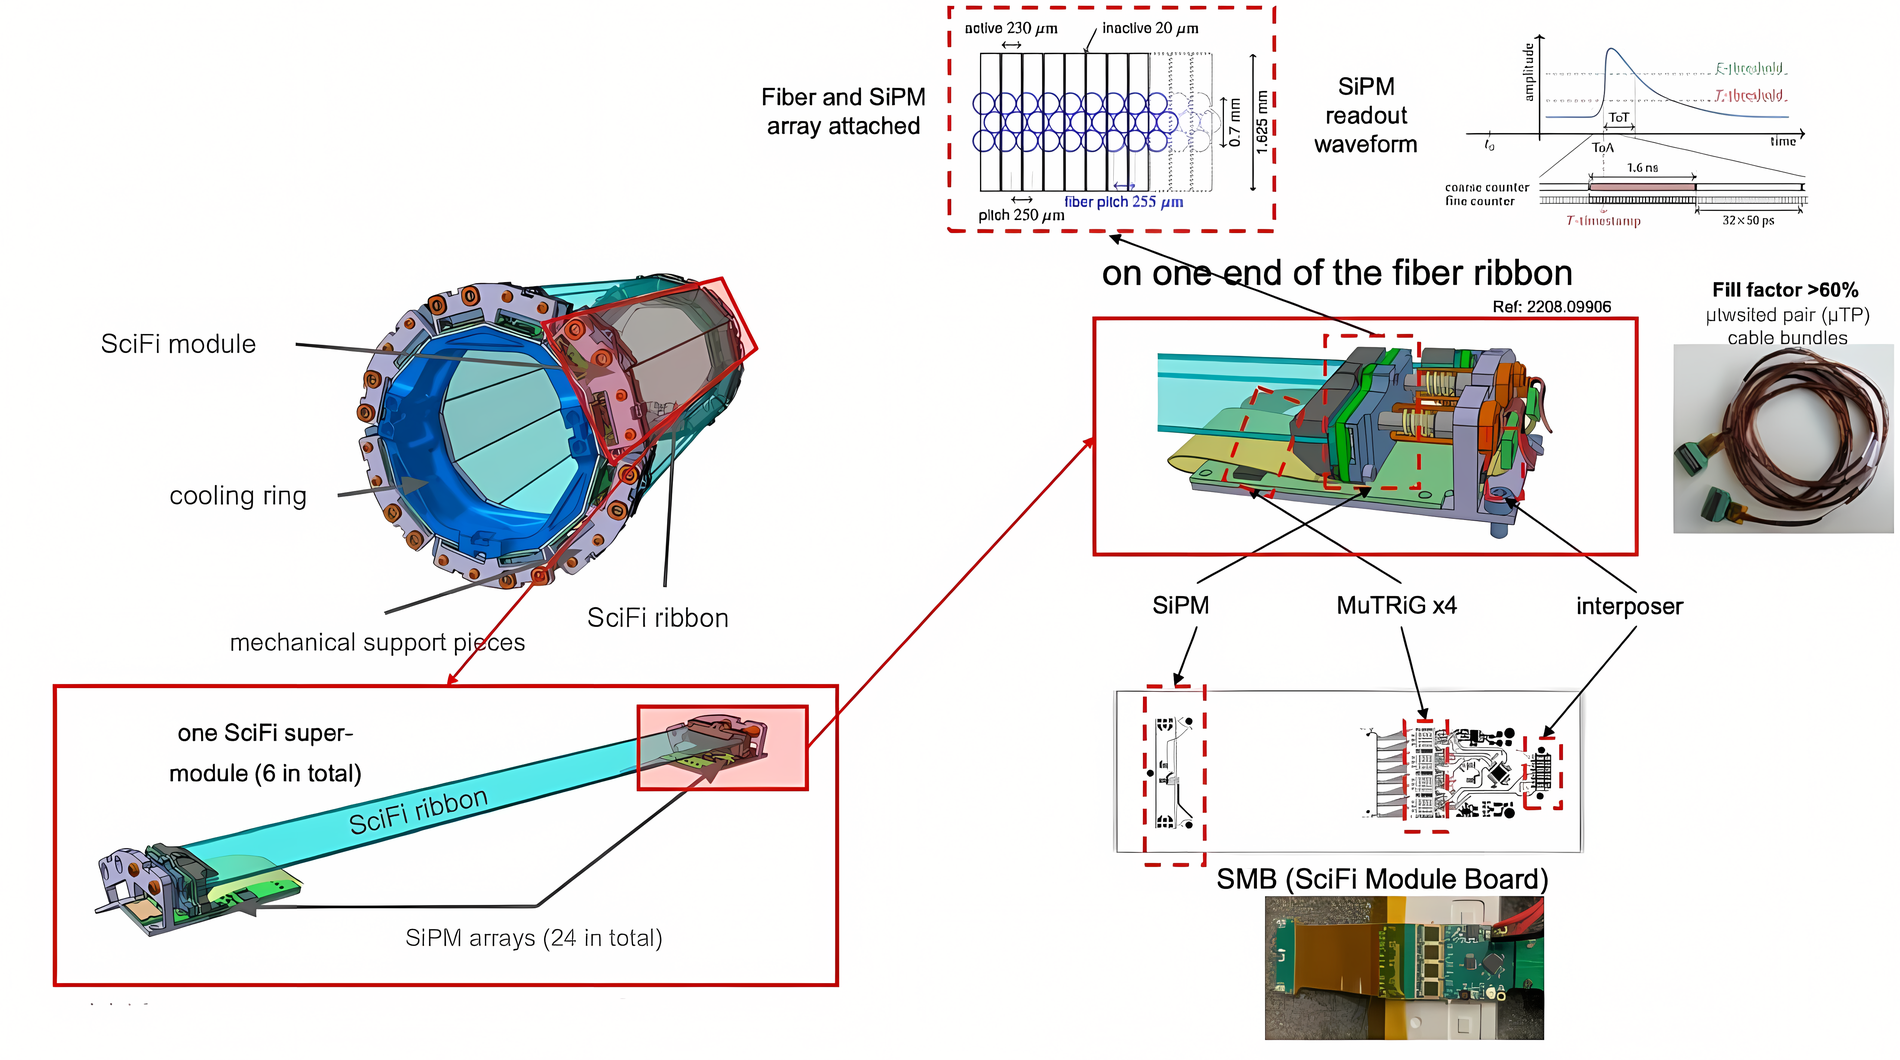
\includegraphics[width=\the\paperwidth-14mm]{../imgs/scifi_modularity.png}};
  \end{tikzpicture}%
}
\begin{frame}{The SciFi detector}
\end{frame}
}

% ====================================================================
% ====================================================================
%  PART II -- the SciFi control and monitoring system: what I built
% ====================================================================
% ====================================================================

% ==================================================================
\section{Overview}
% ==================================================================

\begin{frame}{When I started}
  That's the physics. \textbf{The rest is my own work}: the SciFi control system, built end to end for the PSI run this October.
  \medskip
  \begin{columns}[onlytextwidth,c]
    \begin{column}{0.46\textwidth}
      \small
      \begin{itemize}\setlength{\itemsep}{8pt}
        \item Old page \texttt{Scifi-monitor.js}: grew organically, worked, but \textbf{\textcolor{calcolor}{hard to trust}}, hard to extend.
        \item Replaced end to end: \textbf{\textcolor{metacolor}{Python scripts}} driving the detector $+$ a new \textbf{\textcolor{uicolor}{custom page}} a shifter can rely on.
        \item What follows: \textbf{\textcolor{instcolor}{installation}}, \textbf{\textcolor{uicolor}{interface}}, \textbf{\textcolor{confcolor}{configuration}}, \textbf{\textcolor{calcolor}{calibration}}, \textbf{\textcolor{savecolor}{saving}}.
      \end{itemize}
    \end{column}
    \begin{column}{0.52\textwidth}
      \begin{center}
      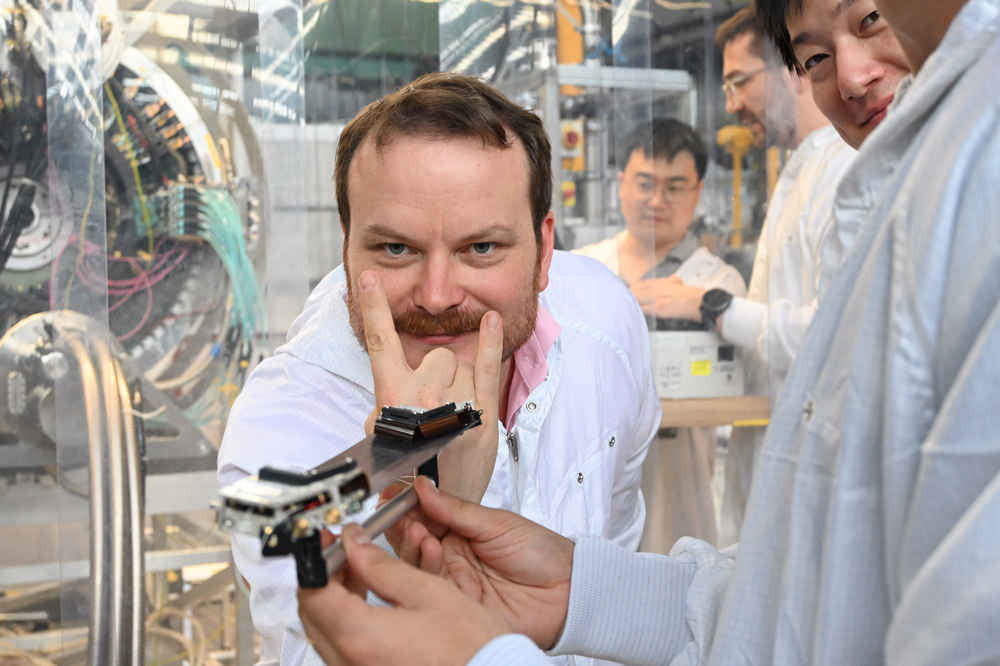
\includegraphics[width=\linewidth]{../imgs/img_context_team.png}
      \end{center}
    \end{column}
  \end{columns}
\end{frame}

\begin{frame}{Where we were $\rightarrow$ where we are}
  \vspace{-6mm}
  \begin{columns}[onlytextwidth,c]
    \begin{column}{0.3\textwidth}
      \begin{center}
      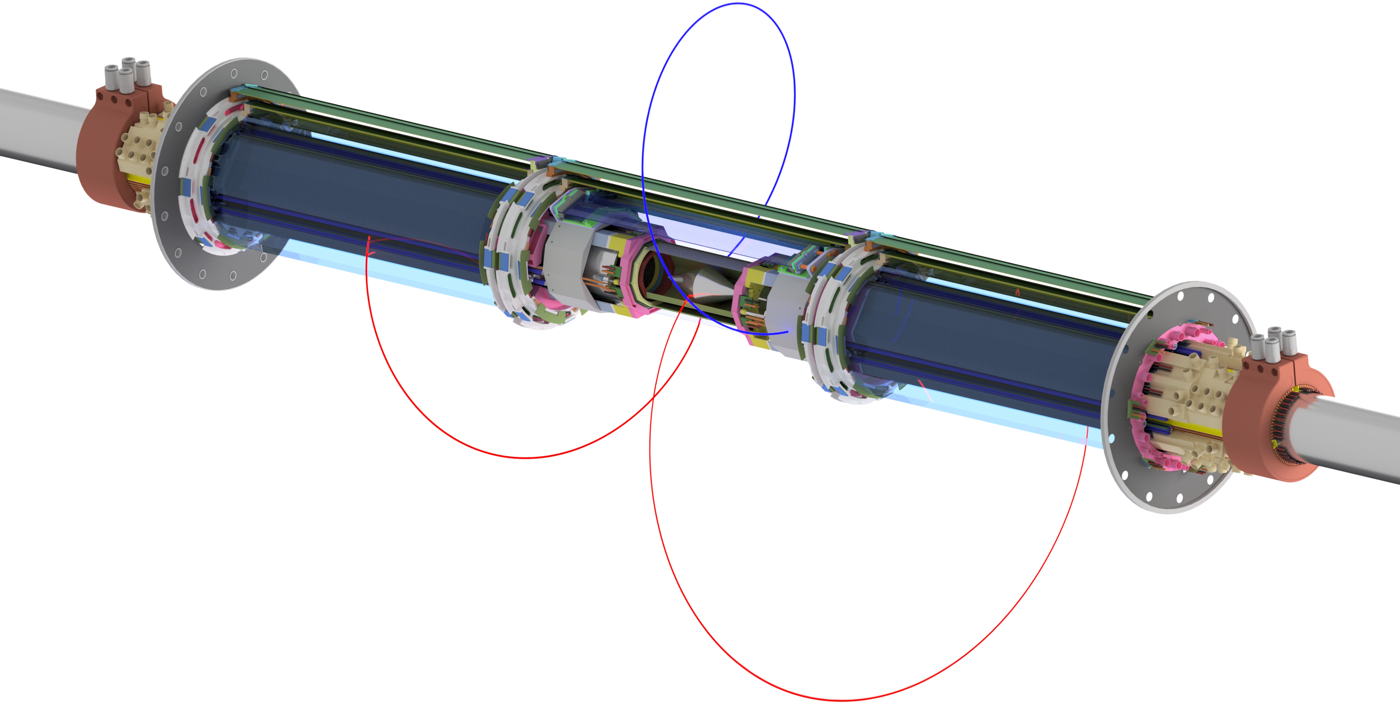
\includegraphics[width=\linewidth]{../imgs/img_scifi.png}

      \bigskip
      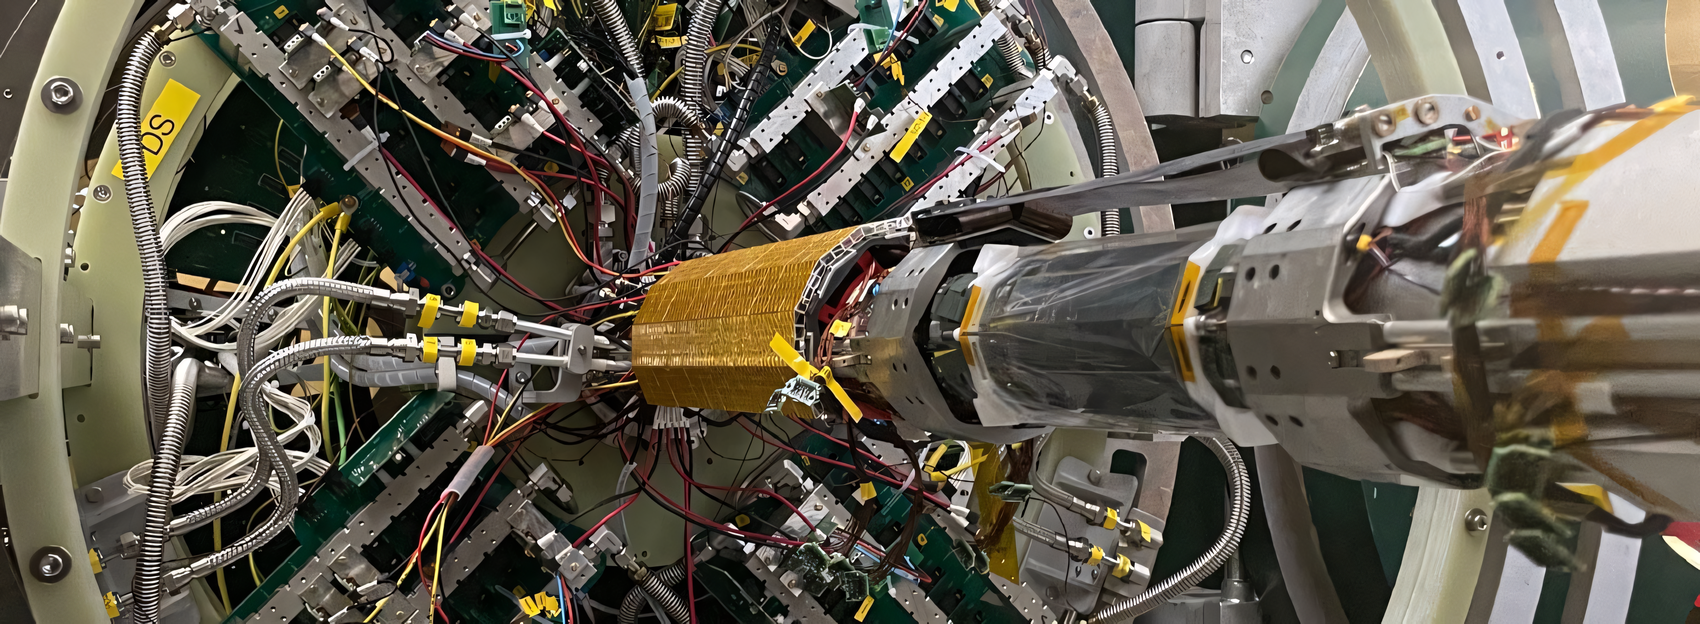
\includegraphics[width=\linewidth]{../imgs/img_mu3e.png}
      \end{center}
    \end{column}
    \begin{column}{0.66\textwidth}
      \begin{center}
      \resizebox{0.82\linewidth}{!}{%
      \begin{tikzpicture}[every node/.style={font=\small}]
        \node[rounded corners, minimum width=2.9cm, minimum height=0.5cm, fill=ETHGray!28,             draw=ETHGray,             thick] (f0) at (0,0)    {};
        \node[rounded corners, minimum width=2.9cm, minimum height=0.5cm, fill=ETHGray!72!ETHBlue!32,   draw=ETHGray!72!ETHBlue,  thick] (f1) at (0,0.54) {};
        \node[rounded corners, minimum width=2.9cm, minimum height=0.5cm, fill=ETHGray!52!ETHBlue!32,   draw=ETHGray!52!ETHBlue,  thick] (f2) at (0,1.08) {};
        \node[rounded corners, minimum width=2.9cm, minimum height=0.5cm, fill=ETHGray!37!ETHBlue!32,   draw=ETHGray!37!ETHBlue,  thick] (f3) at (0,1.62) {};
        \node[rounded corners, minimum width=2.9cm, minimum height=0.5cm, fill=ETHGray!25!ETHBlue!32,   draw=ETHGray!25!ETHBlue,  thick] (f4) at (0,2.16) {};
        \node[rounded corners, minimum width=2.9cm, minimum height=0.5cm, fill=ETHGray!16!ETHBlue!32,   draw=ETHGray!16!ETHBlue,  thick] (f5) at (0,2.70) {};
        \node[rounded corners, minimum width=2.9cm, minimum height=0.5cm, fill=ETHGray!8!ETHBlue!32,    draw=ETHGray!8!ETHBlue,   thick] (f6) at (0,3.24) {};
        \node[rounded corners, minimum width=2.9cm, minimum height=0.5cm, fill=ETHBlue!28,              draw=ETHBlue,             thick] (f7) at (0,3.78) {};

        \node[anchor=west, text=ETHGray]              at ([xshift=3mm]f0.east) {No control system};
        \node[anchor=west, text=ETHGray!72!ETHBlue]   at ([xshift=3mm]f1.east) {Installation};
        \node[anchor=west, text=ETHGray!52!ETHBlue]   at ([xshift=3mm]f2.east) {User Interface};
        \node[anchor=west, text=ETHGray!37!ETHBlue]   at ([xshift=3mm]f3.east) {Power};
        \node[anchor=west, text=ETHGray!25!ETHBlue]   at ([xshift=3mm]f4.east) {Configuration};
        \node[anchor=west, text=ETHGray!16!ETHBlue]   at ([xshift=3mm]f5.east) {Calibration};
        \node[anchor=west, text=ETHGray!8!ETHBlue]    at ([xshift=3mm]f6.east) {Saving};
        \node[anchor=west, text=ETHBlue]              at ([xshift=3mm]f7.east) {New page + full control system};
      \end{tikzpicture}%
      }
      \end{center}
    \end{column}
  \end{columns}
  \bigskip
  \small From an \textbf{ad-hoc JavaScript page} and a handful of disconnected scripts to a \textbf{\textcolor{ETHBlue!65!black}{complete control and monitoring system}} -- built one floor at a time, this is the path the rest of the talk follows.
  \begin{tikzpicture}[remember picture, overlay]
    \draw[densely dashed, thick, ETHBlue!50, -{Stealth[length=2.5mm]}]
      ($(current page.south west)+(0.27\paperwidth,0.46\paperheight)$) to[bend right=12]
      ($(current page.south west)+(0.513\paperwidth,0.402\paperheight)$);
    \draw[densely dashed, thick, ETHBlue!50, -{Stealth[length=2.5mm]}]
      ($(current page.south west)+(0.196\paperwidth,0.714\paperheight)$) to[bend left=12]
      ($(current page.south west)+(0.513\paperwidth,0.798\paperheight)$);
  \end{tikzpicture}
\end{frame}

% ==================================================================
\dividerframe{ETHGray!72!ETHBlue}{1}{Installation}
\section{Installation}
% ==================================================================

\begin{frame}{A week of installation at PSI}
  \vspace{-3mm}
  \noindent\makebox[\linewidth]{%
    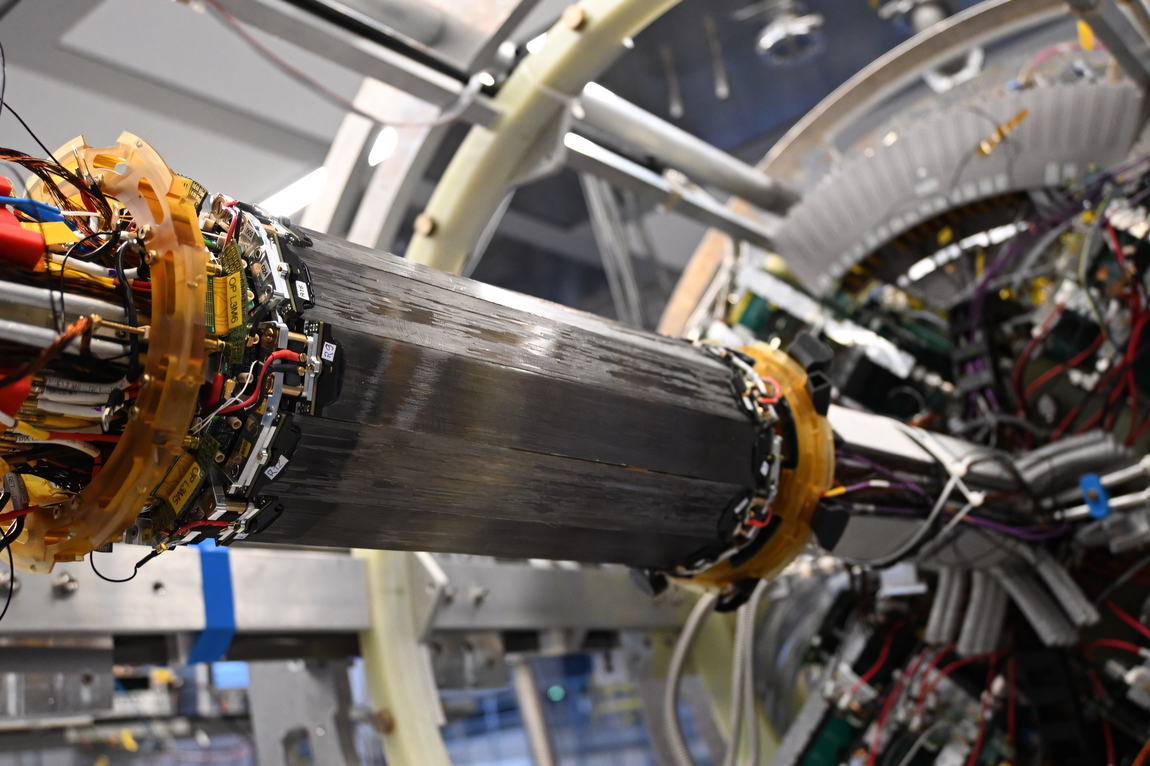
\includegraphics[width=0.4927\linewidth]{../imgs/img_install_wiring.png}\hfill
    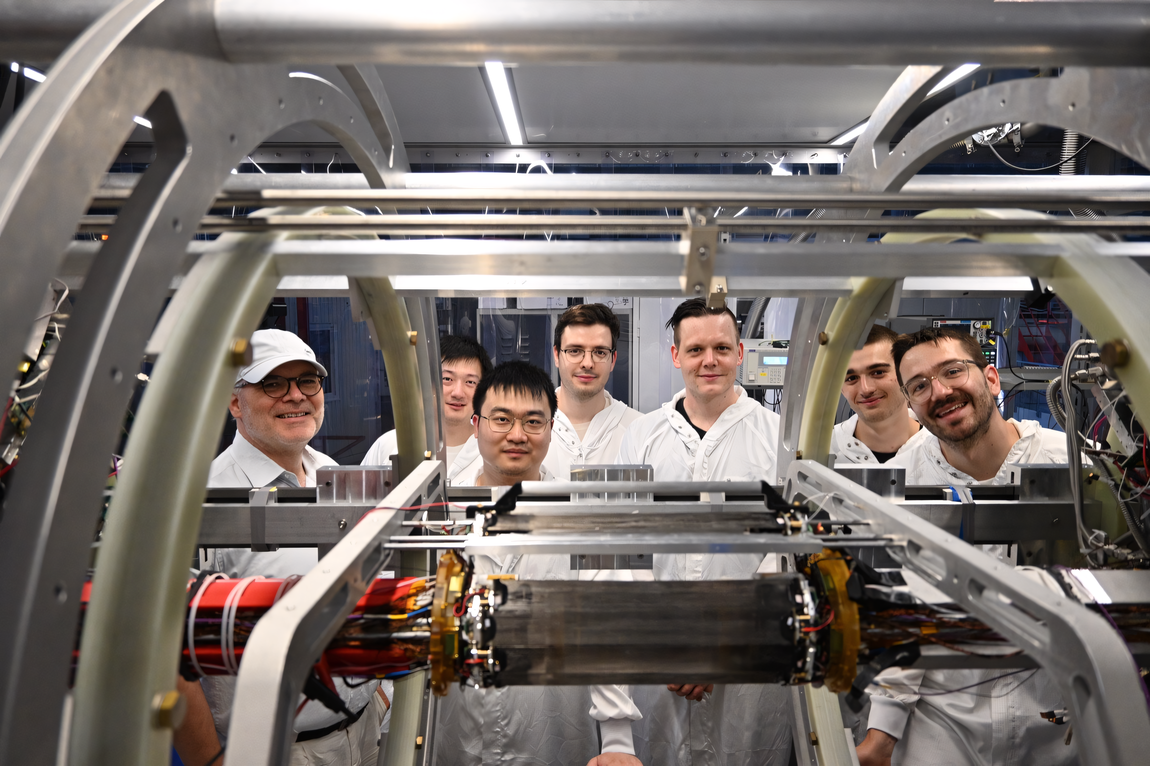
\includegraphics[width=0.4927\linewidth]{../imgs/img_team.png}}\par
  \vspace{1mm}
  \noindent\makebox[\linewidth]{%
    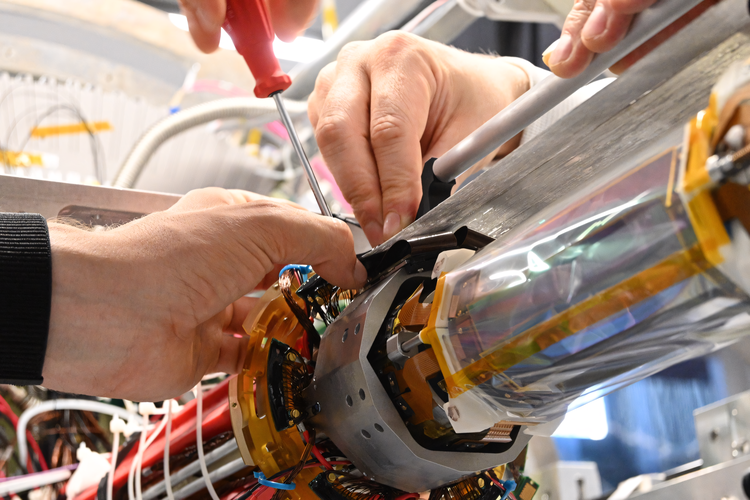
\includegraphics[width=0.239\linewidth]{../imgs/img_install_detail.png}\hfill
    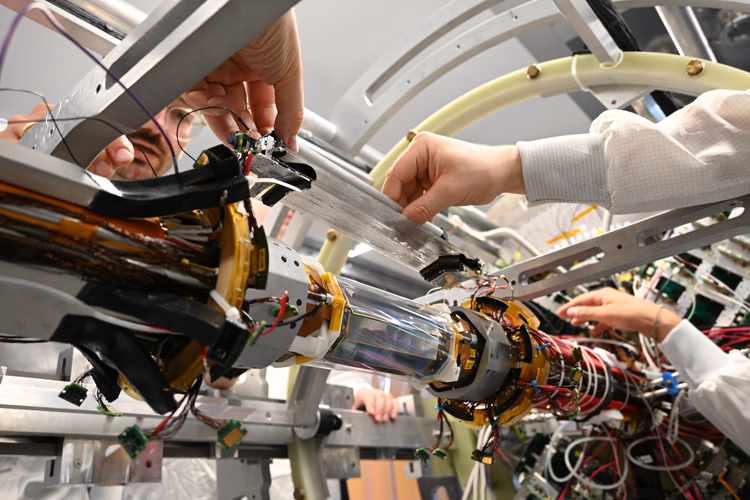
\includegraphics[width=0.239\linewidth]{../imgs/img_install_4.png}\hfill
    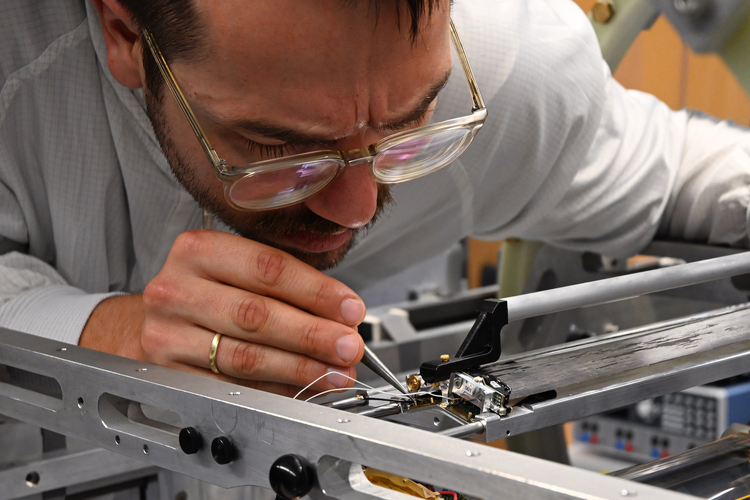
\includegraphics[width=0.239\linewidth]{../imgs/img_install_5.png}\hfill
    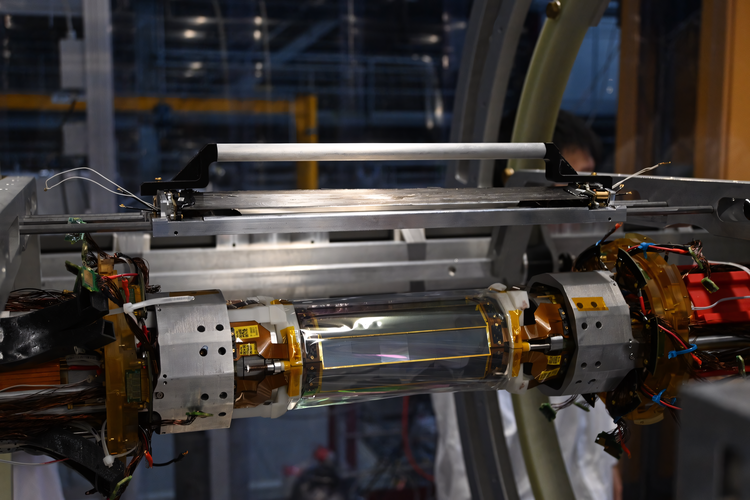
\includegraphics[width=0.239\linewidth]{../imgs/img_install_6.png}}\par
\end{frame}

\begin{frame}{Two chains, one question}
  \vspace{-4mm}
  \begin{center}
  \resizebox{0.92\linewidth}{!}{%
  \begin{tikzpicture}[node distance=6mm, every node/.style={align=center, rounded corners, thick, font=\small,
        minimum width=2.3cm, minimum height=0.85cm}]
    \node[fill=pwrcolor!22, draw=pwrcolor, text=pwrcolor] (p1) {\textbf{Shared}\\power};
    \node[fill=pwrcolor!22, draw=pwrcolor, text=pwrcolor, right=of p1] (p2) {\textbf{Crate}\\status};
    \node[fill=pwrcolor!22, draw=pwrcolor, text=pwrcolor, right=of p2] (p3) {\textbf{Module}\\supply};
    \node[fill=pwrcolor!22, draw=pwrcolor, text=pwrcolor, right=of p3] (p4) {\textbf{Board}\\power};

    \node[fill=uicolor!20, draw=uicolor, text=uicolor, below=22mm of p1] (r1) {\textbf{Readout}\\enabled};
    \node[fill=uicolor!20, draw=uicolor, text=uicolor, right=of r1] (r2) {\textbf{Run}\\active};
    \node[fill=uicolor!20, draw=uicolor, text=uicolor, right=of r2] (r3) {\textbf{Data}\\rate};
    \node[fill=uicolor!20, draw=uicolor, text=uicolor, right=of r3] (r4) {No \textbf{data}\\lost};

    \node[circle, fill=metacolor, text=white, minimum width=1.9cm, minimum height=1.9cm, font=\bfseries\small, right=18mm of p4, yshift=-11mm] (q) {Data\\flowing?};

    \draw[arr] (p1) to[bend left=15]  (p2);
    \draw[arr] (p2) to[bend right=15] (p3);
    \draw[arr] (p3) to[bend left=15]  (p4);
    \draw[arr] (r1) to[bend right=15] (r2);
    \draw[arr] (r2) to[bend left=15]  (r3);
    \draw[arr] (r3) to[bend right=15] (r4);
    \draw[arr] (p4) to[bend right=15] (q);
    \draw[arr] (r4) to[bend left=15]  (q);

    \node[font=\scriptsize\itshape, text=pwrcolor, below=2mm of p1, align=center] {crate \textbf{mains} OK};
    \node[font=\scriptsize\itshape, text=pwrcolor, below=2mm of p2, align=center] {\textbf{DCDC} enabled};
    \node[font=\scriptsize\itshape, text=pwrcolor, below=2mm of p3, align=center] {LV per \textbf{module}};
    \node[font=\scriptsize\itshape, text=pwrcolor, below=2mm of p4, align=center] {\textbf{FEB} power good};
    \node[font=\scriptsize\itshape, text=uicolor, above=2mm of r1, align=center] {\textbf{frontend} armed};
    \node[font=\scriptsize\itshape, text=uicolor, above=2mm of r2, align=center] {\textbf{MIDAS} run started};
    \node[font=\scriptsize\itshape, text=uicolor, above=2mm of r3, align=center] {$>$0\,Hz per \textbf{FEB}};
    \node[font=\scriptsize\itshape, text=uicolor, above=2mm of r4, align=center] {\textbf{buffers} not full};
  \end{tikzpicture}%
  }
  \end{center}
  \small Two chains, checked separately -- \textcolor{pwrcolor}{\textbf{power}} can be all green while \textcolor{uicolor}{\textbf{readout}} stays idle.\\Only when both agree does data actually flow.
\end{frame}

% ==================================================================
\dividerframe{ETHGray!52!ETHBlue}{2}{User Interface}
\section{User Interface}
% ==================================================================

\begin{frame}{From hardware to shifter}
  \begin{columns}[onlytextwidth,c]
    \begin{column}{0.56\textwidth}
      \begin{itemize}\small\setlength{\itemsep}{8pt}
        \item The chain runs \textbf{both ways}: status flows up to the shifter, \textbf{\textcolor{uicolor}{changes}} flow back down --- some only apply at a trigger point (e.g.\ run start).
        \item \alert{Nothing is ever hard-blocked}: every action stays clickable; the page warns instead of stopping you.
        \item \textbf{MIDAS} ties it together --- frontends, ODB and this page all run inside it.
      \end{itemize}
    \end{column}
    \begin{column}{0.4\textwidth}
      \begin{center}
      \resizebox{!}{0.75\textheight}{%
      \begin{tikzpicture}[node distance=5mm]
        \node[boxhw] (hw) {Detector};
        \node[boxhw, below=of hw] (fe) {Frontends};
        \node[boxhw, below=of fe] (odb) {ODB\\\footnotesize(online database)};
        \node[boxui, below=of odb] (page) {Custom page};
        \node[boxui, below=of page] (user) {Shifter};
        \foreach \a/\b in {hw/fe, fe/odb, odb/page, page/user}
          \draw[{Stealth[length=2.2mm]}-{Stealth[length=2.2mm]}, thick, draw=ETHGray] (\a) -- (\b);
        \begin{pgfonlayer}{background}
          \node[fill=ETHBlue!8, draw=ETHBlue!40, thick, rounded corners=1.5pt,
                fit=(hw)(fe)(odb)(page)(user), inner xsep=8mm, inner ysep=3mm] (midasbg) {};
        \end{pgfonlayer}
        \node[font=\small\itshape, text=ETHBlue!55!black, rotate=90, xshift=7mm] at (midasbg.west) {MIDAS};
      \end{tikzpicture}%
      }
      \end{center}
    \end{column}
  \end{columns}
\end{frame}

\begin{frame}{The page: then and now}
  \begin{columns}[onlytextwidth,T]
    \begin{column}{0.46\textwidth}
      \vspace{-5mm}
      \begin{flushleft}
      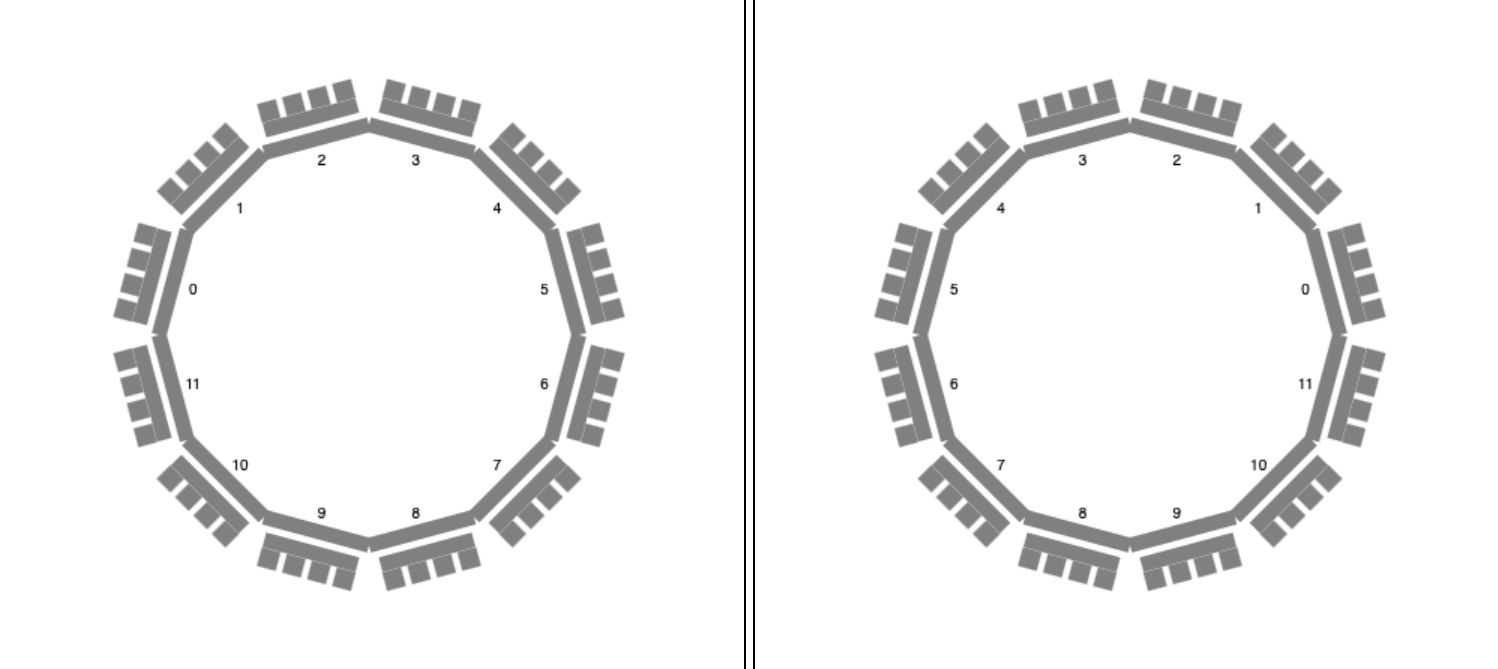
\includegraphics[width=0.97\linewidth]{../imgs/img_page_old.png}
      \end{flushleft}
      \begin{center}
      \vspace{-3mm}
      \href{http://localhost:8080/?cmd=custom&page=SciFi\%20Main}{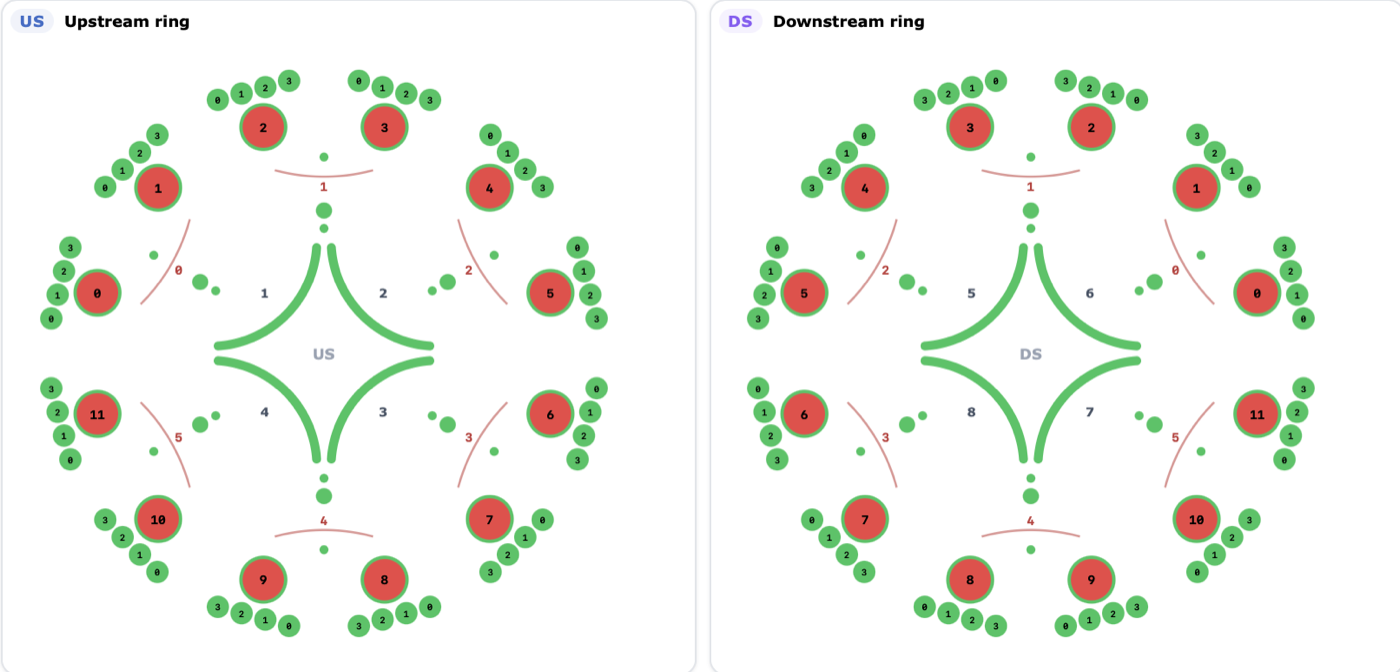
\includegraphics[width=0.97\linewidth]{../imgs/img_page_new.png}}
      \end{center}
    \end{column}
    \begin{column}{0.5\textwidth}
      \vspace{2mm}
      \small
      \begin{itemize}\setlength{\itemsep}{7pt}
        \item Old page: a static, unlabeled ring --- \textbf{\textcolor{calcolor}{no live status}}, nothing clickable.
        \item New page splits in two: \textbf{\textcolor{uicolor}{Geometry}} read-only diagnostic; \textbf{\textcolor{pwrcolor}{Power}} / \textbf{\textcolor{uicolor}{Readout}} / \textbf{\textcolor{calcolor}{Calibration}} the only editable surface.
        \item Each value goes to \textbf{\textcolor{savecolor}{ODB}} --- a frontend pushes it onto the hardware.
        \item Safety logic stays in \textbf{\textcolor{metacolor}{Python}}, never duplicated in JavaScript.
      \end{itemize}
    \end{column}
  \end{columns}
\end{frame}

% ==================================================================
\dividerframe{ETHGray!37!ETHBlue}{3}{Power}
\section{Power}
% ==================================================================

\begin{frame}{From detector to Power and Readout}
  \begin{columns}[onlytextwidth,T]
    \begin{column}{0.56\textwidth}
      \begin{center}
      \resizebox{!}{0.65\textheight}{%
      \begin{tikzpicture}[every node/.style={align=center, rounded corners, thick,
            minimum width=2.6cm, minimum height=0.9cm, font=\small}]
        \node[fill=ETHGray!12,   draw=ETHGray,   text=ETHGray!70!black]   (tdk)  at (0,0)       {TDK};
        \node[fill=ETHGray!12,   draw=ETHGray,   text=ETHGray!70!black]   (pd)   at (0,-1.3)    {PowerDist};
        \node[fill=pwrcolor!22,  draw=pwrcolor,  text=pwrcolor]  (dcdc) at (-3.0,-2.6) {DCDC crates};
        \node[fill=ETHGray!12,   draw=ETHGray,   text=ETHGray!70!black]   (fe)   at (3.0,-2.6)  {Frontend};
        \node[fill=pwrcolor!22,  draw=pwrcolor,  text=pwrcolor]  (lvch) at (-3.0,-3.9) {LV channels};
        \node[fill=metacolor!22, draw=metacolor, text=metacolor] (feb)  at (1.2,-3.9)  {FEB};
        \node[fill=calcolor!22,  draw=calcolor,  text=calcolor]  (hvch) at (4.6,-3.9)  {HV channels};
        \node[fill=uicolor!22,   draw=uicolor,   text=uicolor]   (rout) at (-0.2,-5.4) {Readout};
        \node[fill=calcolor!22,  draw=calcolor,  text=calcolor]  (sipm) at (3.3,-5.4)  {SiPM};
        \node[fill=uicolor!22,   draw=uicolor,   text=uicolor]   (ready) at (1.55,-6.8) {Detector};

        \draw[-{Stealth[length=2.2mm]}, thick, ETHGray!55]   (tdk) -- (pd);
        \draw[-{Stealth[length=2.2mm]}, thick, ETHGray!55]   (pd) to[bend right=20] (dcdc);
        \draw[-{Stealth[length=2.2mm]}, thick, ETHGray!55]   (pd) to[bend left=20] (fe);
        \draw[-{Stealth[length=2.2mm]}, thick, pwrcolor!80]  (dcdc) -- (lvch);
        \draw[-{Stealth[length=2.2mm]}, thick, ETHGray!55]   (fe) to[bend left=15] (hvch);
        \draw[-{Stealth[length=2.2mm]}, thick, ETHGray!55]   (fe) to[bend right=15] (feb);
        \draw[-{Stealth[length=2.2mm]}, thick, pwrcolor!80]  (lvch) to[bend left=15] (rout);
        \draw[-{Stealth[length=2.2mm]}, thick, metacolor!80] (feb) to[bend right=15] (rout);
        \draw[-{Stealth[length=2.2mm]}, thick, calcolor!80]  (hvch) to[bend right=10] (sipm);
        \draw[-{Stealth[length=2.2mm]}, thick, uicolor!80]   (rout) to[bend left=10] (ready);
        \draw[-{Stealth[length=2.2mm]}, thick, calcolor!80]  (sipm) to[bend right=10] (ready);
      \end{tikzpicture}%
      }
      \end{center}
    \end{column}
    \begin{column}{0.4\textwidth}
      \begin{itemize}\small\setlength{\itemsep}{6pt}
        \item \textbf{\textcolor{ETHGray!70!black}{TDK}} and \textbf{\textcolor{ETHGray!70!black}{PowerDist}} -- the same first two devices for all three chains.
        \item \textbf{\textcolor{pwrcolor}{LV}} -- through its own \textbf{\textcolor{pwrcolor}{DCDC crates}} -- feeds the \textbf{\textcolor{uicolor}{Readout}}.
        \item \textbf{\textcolor{calcolor}{HV}} and \textbf{\textcolor{metacolor}{FEB}} both wait for their \textbf{\textcolor{ETHGray!70!black}{Frontend}}.
        \item \textbf{\textcolor{calcolor}{HV}} feeds the \textbf{\textcolor{calcolor}{SiPM}}; \textbf{\textcolor{metacolor}{FEB}} feeds the \textbf{\textcolor{uicolor}{Readout}} too.
        \item \textbf{\textcolor{uicolor}{Readout}} and \textbf{\textcolor{calcolor}{SiPM}} both lead back to the \textbf{\textcolor{uicolor}{detector}}.
      \end{itemize}
    \end{column}
  \end{columns}
\end{frame}

% ==================================================================
\dividerframe{ETHGray!25!ETHBlue}{4}{Configuration}
\section{Configuration}
% ==================================================================

\begin{frame}{Configuration: one hub, four jobs}
  \begin{center}
  \resizebox{0.88\linewidth}{!}{%
  \begin{tikzpicture}[every node/.style={align=center, rounded corners=4pt, line width=1pt, font=\small}]
    \node[fill=ETHGray!10, draw=ETHGray!60, text=ETHGray!70!black, minimum width=3.0cm, minimum height=1.0cm] (start) at (0,0) {\textbf{Configuration}};

    \node[fill=confcolor!18, draw=confcolor, text=confcolor, minimum width=3.4cm, minimum height=1.15cm] (paramalg) at (-5.6,-2.1) {Walk \textbf{FEB} $\to$ module\\$\to$ chip $\to$ channel};
    \node[fill=calcolor!18,  draw=calcolor,  text=calcolor,  minimum width=3.4cm, minimum height=1.15cm] (pllalg)   at (-1.87,-2.1) {Verify \textbf{clock}\\recovery};
    \node[fill=metacolor!18, draw=metacolor, text=metacolor, minimum width=3.4cm, minimum height=1.15cm] (prbsalg)  at (1.87,-2.1)  {Check \textbf{link}\\integrity};
    \node[fill=uicolor!18,   draw=uicolor,   text=uicolor,   minimum width=3.4cm, minimum height=1.15cm] (tdcalg)   at (5.6,-2.1)  {Verify \textbf{per-channel}\\test pulse};

    \node[fill=confcolor!18, draw=confcolor, text=confcolor, minimum width=2.8cm, minimum height=0.9cm] (param) at (-5.6,-3.8) {\textbf{Parameters}\\(ODB tree)};
    \node[fill=calcolor!18,  draw=calcolor,  text=calcolor,  minimum width=2.6cm, minimum height=0.9cm] (pll)   at (-1.87,-3.8) {\textbf{PLL} test};
    \node[fill=metacolor!18, draw=metacolor, text=metacolor, minimum width=2.6cm, minimum height=0.9cm] (prbs)  at (1.87,-3.8)  {\textbf{PRBS} test};
    \node[fill=uicolor!18,   draw=uicolor,   text=uicolor,   minimum width=2.6cm, minimum height=0.9cm] (tdc)   at (5.6,-3.8)  {\textbf{TDC} test};

    \draw[-{Stealth[length=2.2mm]}, thick, confcolor!80]  (start) to[bend right=20] (paramalg);
    \draw[-{Stealth[length=2.2mm]}, thick, calcolor!80]   (start) to[bend right=9]  (pllalg);
    \draw[-{Stealth[length=2.2mm]}, thick, metacolor!80]  (start) to[bend left=9]   (prbsalg);
    \draw[-{Stealth[length=2.2mm]}, thick, uicolor!80]    (start) to[bend left=20]  (tdcalg);
    \draw[-{Stealth[length=2.2mm]}, thick, confcolor!80]  (paramalg) to[bend left=8]  (param);
    \draw[-{Stealth[length=2.2mm]}, thick, calcolor!80]   (pllalg)   to[bend right=8] (pll);
    \draw[-{Stealth[length=2.2mm]}, thick, metacolor!80]  (prbsalg)  to[bend left=8]  (prbs);
    \draw[-{Stealth[length=2.2mm]}, thick, uicolor!80]    (tdcalg)   to[bend right=8] (tdc);
  \end{tikzpicture}%
  }
  \end{center}
  \smallskip
  \small \textcolor{confcolor}{\textbf{Configuration}} has grown beyond parameter editing into the detector's general hardware test hub -- the old \textbf{Readout} tab folds in here entirely, and every parameter still writes to a dedicated \textbf{ODB} tree, read directly by the Python scripts.
\end{frame}

% ==================================================================
\dividerframe{ETHGray!16!ETHBlue}{5}{Calibration}
\section{Calibration}
% ==================================================================

\begin{frame}{Two calibrations, one starting point}
  \begin{center}
  \resizebox{0.66\linewidth}{!}{%
  \begin{tikzpicture}[every node/.style={align=center, rounded corners=4pt, line width=1pt, font=\small}]
    \node[fill=ETHGray!10, draw=ETHGray!60, text=ETHGray!70!black, minimum width=2.8cm, minimum height=1.0cm] (start) at (0,0) {\textbf{Start}};

    \node[fill=calcolor!18, draw=calcolor, text=calcolor, minimum width=3.6cm, minimum height=1.2cm] (thralg) at (-2.6,-2.0) {Walk \textbf{threshold},\\read rate curve};
    \node[fill=pwrcolor!18, draw=pwrcolor, text=pwrcolor, minimum width=3.6cm, minimum height=1.2cm] (vbralg) at (2.6,-2.0)   {\textbf{Derivative} $+$\\Gaussian fit};

    \node[fill=calcolor!18, draw=calcolor, text=calcolor, minimum width=2.8cm, minimum height=0.9cm] (thr) at (-2.6,-3.7) {\textbf{ScanThr}};
    \node[fill=pwrcolor!18, draw=pwrcolor, text=pwrcolor, minimum width=2.8cm, minimum height=0.9cm] (vbr) at (2.6,-3.7)    {\textbf{ScanVbr}};

    \draw[-{Stealth[length=2.2mm]}, thick, calcolor!80] (start) to[bend right=18] (thralg);
    \draw[-{Stealth[length=2.2mm]}, thick, pwrcolor!80] (start) to[bend left=18]  (vbralg);
    \draw[-{Stealth[length=2.2mm]}, thick, calcolor!80] (thralg) to[bend left=8]  (thr);
    \draw[-{Stealth[length=2.2mm]}, thick, pwrcolor!80] (vbralg) to[bend right=8] (vbr);
  \end{tikzpicture}%
  }
  \end{center}
  \smallskip
  \small Both share the same \texttt{CalibrationBase} lifecycle -- \textbf{prepare}, \textbf{execute}, \textbf{finalise}.
\end{frame}

\begin{frame}{How a calibration actually runs}
  \begin{columns}[onlytextwidth,T]
    \begin{column}{0.32\textwidth}
      \begin{itemize}\small\setlength{\itemsep}{6pt}
        \item \textbf{\textcolor{uicolor}{Start}} -- the page writes ODB and hands off to PySequencer.
        \item \textbf{\textcolor{metacolor}{Script}} -- PySequencer launches it, it connects to MIDAS.
        \item \textbf{\textcolor{calcolor}{Lifecycle}} -- prepare, execute, finalise.
        \item \textbf{\textcolor{savecolor}{Save}} -- result written to ODB, local, and CDB.
        \item \textbf{\textcolor{uicolor}{Result}} -- the page shows it back to the shifter.
      \end{itemize}
    \end{column}
    \begin{column}{0.63\textwidth}
  \begin{center}
  \resizebox{\linewidth}{!}{%
  \begin{tikzpicture}[node distance=4.5mm, every node/.style={align=center, rounded corners, thick, font=\small}]
    \node[fill=uicolor!22,   draw=uicolor,   text=uicolor,   minimum width=4.2cm] (start) {Shifter presses Start};
    \node[fill=uicolor!22,   draw=uicolor,   text=uicolor,   minimum width=4.2cm, below=of start] (odbw) {Page writes ODB};
    \node[fill=metacolor!22, draw=metacolor, text=metacolor, minimum width=4.2cm, below=of odbw] (pyseq) {PySequencer picks up script};
    \node[fill=metacolor!22, draw=metacolor, text=metacolor, minimum width=4.2cm, below=of pyseq] (script) {Script connects to MIDAS};
    \node[fill=calcolor!22, draw=calcolor, text=calcolor, minimum width=1.7cm, below=7mm of script, xshift=-2.4cm] (prep) {Prepare};
    \node[fill=calcolor!22, draw=calcolor, text=calcolor, minimum width=1.7cm, below=7mm of script] (exec) {Execute};
    \node[fill=calcolor!22, draw=calcolor, text=calcolor, minimum width=1.7cm, below=7mm of script, xshift=2.4cm] (fin) {Finalise};
    \node[fill=savecolor!22, draw=savecolor, text=savecolor, minimum width=2.1cm, below=7mm of fin, xshift=-2.6cm] (odb) {ODB (live)};
    \node[fill=savecolor!22, draw=savecolor, text=savecolor, minimum width=2.1cm, below=7mm of fin] (local) {Local (recent)};
    \node[fill=savecolor!22, draw=savecolor, text=savecolor, minimum width=2.1cm, below=7mm of fin, xshift=2.9cm] (cdb) {CDB (permanent)};
    \node[fill=uicolor!22, draw=uicolor, text=uicolor, minimum width=4.2cm, below=7mm of local] (result) {Page shows the result};

    \draw[-{Stealth[length=2.2mm]}, thick, ETHGray!55] (start) -- (odbw);
    \draw[-{Stealth[length=2.2mm]}, thick, ETHGray!55] (odbw) -- (pyseq);
    \draw[-{Stealth[length=2.2mm]}, thick, ETHGray!55] (pyseq) -- (script);
    \draw[-{Stealth[length=2.2mm]}, thick, ETHGray!55] (script) to[bend right=15] (prep);
    \draw[-{Stealth[length=2.2mm]}, thick, ETHGray!55] (prep) to[bend left=15] (exec);
    \draw[-{Stealth[length=2.2mm]}, thick, ETHGray!55] (exec) to[bend left=15] (fin);
    \draw[-{Stealth[length=2.2mm]}, thick, ETHGray!55] (fin) to[bend right=20] (odb);
    \draw[-{Stealth[length=2.2mm]}, thick, ETHGray!55] (fin) -- (local);
    \draw[-{Stealth[length=2.2mm]}, thick, ETHGray!55] (fin) to[bend left=20]  (cdb);
    \draw[-{Stealth[length=2.2mm]}, thick, ETHGray!55] (odb) to[bend right=15] (result);
    \draw[-{Stealth[length=2.2mm]}, thick, ETHGray!55] (local) -- (result);
    \draw[-{Stealth[length=2.2mm]}, thick, ETHGray!55] (cdb) to[bend left=15]  (result);
    \draw[thick, dashed, ETHBlue!50, -{Stealth[length=2.5mm]}] (result.east) to[bend right=70] (start.east);
  \end{tikzpicture}%
  }
  \end{center}
    \end{column}
  \end{columns}
\end{frame}

% ==================================================================
\dividerframe{ETHGray!8!ETHBlue}{6}{Saving}
\section{Saving}
% ==================================================================

\begin{frame}{Saving: ODB, local, and CDB}
  \begin{center}
  \resizebox{0.85\linewidth}{!}{%
  \begin{tikzpicture}[font=\small]
    \node[circle, fill=calcolor!22, draw=calcolor, line width=1pt, minimum size=2.8mm, inner sep=0pt] (scan) at (0,0) {};
    \node[font=\footnotesize, below=2mm, xshift=-9mm, text=calcolor] at (0,0) {\textbf{Scan} result};

    \node[circle, fill=uicolor, minimum size=2.4mm, inner sep=0pt] (bodb) at (3,1.7) {};
    \node[circle, fill=metacolor, minimum size=2.4mm, inner sep=0pt] (blocal) at (3.4,0) {};
    \node[circle, fill=savecolor, minimum size=2.4mm, inner sep=0pt] (bcdb) at (3,-1.7) {};
    \draw[-{Stealth[length=2.2mm]}, thick, uicolor!80]   (scan) to[bend left=15]  (bodb);
    \draw[-{Stealth[length=2.2mm]}, thick, metacolor!80] (scan) -- (blocal);
    \draw[-{Stealth[length=2.2mm]}, thick, savecolor!65] (scan) to[bend right=15] (bcdb);

    \node[font=\small, align=left, anchor=west, text=uicolor] at ([xshift=4mm]bodb) {\textbf{ODB} -- \texttt{ResultSaverROOT}\\\textbf{live} only, overwritten each scan};
    \node[font=\small, align=left, anchor=west, text=metacolor] at ([xshift=4mm]blocal) {\textbf{Local} -- most recent calibration per FEB\\cached on disk, for day-to-day operations};
    \node[font=\small, align=left, anchor=west, text=savecolor] at ([xshift=4mm]bcdb) {\textbf{CDB} -- \texttt{ResultSaverCDB}\\indexed by name + run, \textbf{permanent}};
  \end{tikzpicture}%
  }
  \end{center}
  \smallskip
  \small All three destinations are genuinely wired into the calibration scripts now, which was not true before.
  \smallskip
  \begin{columns}[onlytextwidth,T]
    \begin{column}{0.31\textwidth}
      \begin{itemize}\small
        \item \textbf{\textcolor{uicolor}{ODB}} -- \emph{``What's the calibration right now?''}
      \end{itemize}
    \end{column}
    \begin{column}{0.34\textwidth}
      \begin{itemize}\small
        \item \textbf{\textcolor{metacolor}{Local}} -- \emph{``What did we last calibrate, for operations?''}
      \end{itemize}
    \end{column}
    \begin{column}{0.31\textwidth}
      \begin{itemize}\small
        \item \textbf{\textcolor{savecolor}{CDB}} -- \emph{``What was it on a given run?''}
      \end{itemize}
    \end{column}
  \end{columns}
\end{frame}

% ==================================================================
\dividerframe{ETHBlue}{7}{Big Picture}
\section{Big Picture}
% ==================================================================

\begin{frame}{The work, as a branch diagram}
  It helps to think about this effort the way you'd think about a software repository.
  \begin{center}
  \resizebox{\linewidth}{!}{%
  \begin{tikzpicture}[x=1.3cm, y=1cm]
    \draw[thick, ETHGray!60] (0,0) -- (18,0);
    \node[circle, fill=instcolor!24, draw=instcolor, line width=1pt, minimum size=2.6mm, inner sep=0pt] at (0,0) {};
    \node[circle, fill=uicolor!24,   draw=uicolor,   line width=1pt, minimum size=2.6mm, inner sep=0pt] at (2,0) {};
    \node[circle, fill=pwrcolor!24,  draw=pwrcolor,  line width=1pt, minimum size=2.6mm, inner sep=0pt] at (6,0) {};
    \node[circle, fill=confcolor!24, draw=confcolor, line width=1pt, minimum size=2.6mm, inner sep=0pt] at (10,0) {};
    \node[circle, fill=calcolor!24,  draw=calcolor,  line width=1pt, minimum size=2.6mm, inner sep=0pt] at (14,0) {};
    \node[circle, fill=savecolor!24, draw=savecolor, line width=1pt, minimum size=2.6mm, inner sep=0pt] at (18,0) {};
    \node[font=\footnotesize, below=2mm, text=instcolor]  at (0,0)  {\textbf{Installation}};
    \node[font=\footnotesize, below=2mm, text=uicolor]    at (2,0)  {\textbf{User Interface}};
    \node[font=\footnotesize, below=2mm, text=pwrcolor]   at (6,0)  {\textbf{Power}};
    \node[font=\footnotesize, below=2mm, xshift=7mm,  text=confcolor]  at (10,0) {\textbf{Configuration}};
    \node[font=\footnotesize, below=2mm, xshift=-3mm, text=calcolor]   at (14,0) {\textbf{Calibration}};
    \node[font=\footnotesize, below=2mm, text=savecolor]  at (18,0) {\textbf{Saving}};

    % Installation -> User Interface
    \draw[thick, uicolor!80] (0,0) .. controls (0.6,0.9) and (1.4,0.9) .. (2,0)
      node[pos=0.5, circle, fill=uicolor, minimum size=2.4mm, inner sep=0pt] (page) {};
    \node[font=\scriptsize, above=1mm of page, text=uicolor] {\textbf{Custom page}};

    % User Interface -> Power: three independent bring-up sequences
    \draw[thick, pwrcolor!80] (2,0) .. controls (3.2,1.1) and (4.8,1.1) .. (6,0)
      node[pos=0.22, circle, fill=pwrcolor, minimum size=2.4mm, inner sep=0pt] (lv)  {}
      node[pos=0.5,  circle, fill=pwrcolor, minimum size=2.4mm, inner sep=0pt] (hv)  {}
      node[pos=0.78, circle, fill=pwrcolor, minimum size=2.4mm, inner sep=0pt] (feb) {};
    \node[font=\scriptsize, above=1mm of lv, xshift=3mm, text=pwrcolor] {\textbf{LV} bring-up};
    \node[font=\scriptsize, below=1mm of hv,  text=pwrcolor] {\textbf{HV} bring-up};
    \node[font=\scriptsize, above=1mm of feb, text=pwrcolor] {\textbf{FEB} bring-up};

    % Power -> Configuration: page tabs
    \draw[thick, confcolor!80] (6,0) .. controls (7.2,-1.0) and (8.8,-1.0) .. (10,0)
      node[pos=0.22, circle, fill=confcolor, minimum size=2.4mm, inner sep=0pt] (ptab) {}
      node[pos=0.62, circle, fill=confcolor, minimum size=2.4mm, inner sep=0pt] (gtab) {};
    \node[font=\scriptsize, below=1mm of ptab, text=confcolor] {\textbf{Power} tab};
    \node[font=\scriptsize, below=1mm of gtab, text=confcolor] {\textbf{Geometry} tab};

    % Configuration -> Calibration: hardware test branch
    \draw[thick, calcolor!80] (10,0) .. controls (11.2,1.1) and (12.8,1.1) .. (14,0)
      node[pos=0.22, circle, fill=calcolor, minimum size=2.4mm, inner sep=0pt] (pll)  {}
      node[pos=0.5,  circle, fill=calcolor, minimum size=2.4mm, inner sep=0pt] (prbs) {}
      node[pos=0.78, circle, fill=calcolor, minimum size=2.4mm, inner sep=0pt] (tdc)  {};
    \node[font=\scriptsize, above=1mm of pll,  text=calcolor] {\textbf{PLL} test};
    \node[font=\scriptsize, below=1mm of prbs, text=calcolor] {\textbf{PRBS} test};
    \node[font=\scriptsize, above=1mm of tdc,  text=calcolor] {\textbf{TDC} test};

    % Calibration -> Saving: two independent calibration scans
    \draw[thick, savecolor!65] (14,0) .. controls (15.2,-1.0) and (16.8,-1.0) .. (18,0)
      node[pos=0.25, circle, fill=savecolor, minimum size=2.4mm, inner sep=0pt] (thr) {}
      node[pos=0.75, circle, fill=savecolor, minimum size=2.4mm, inner sep=0pt] (vbr) {};
    \node[font=\scriptsize, below=1mm of thr, text=savecolor] {\textbf{Threshold} scan};
    \node[font=\scriptsize, below=1mm of vbr, text=savecolor] {\textbf{Breakdown} scan};
  \end{tikzpicture}%
  }
  \end{center}
  \bigskip
  A single \textbf{main line} from \textbf{\textcolor{instcolor}{Installation}} to \textbf{\textcolor{savecolor}{Saving}}, with every concrete piece built as a \textbf{branch}: three \textbf{\textcolor{pwrcolor}{bring-up}} sequences, a family of \textbf{\textcolor{calcolor}{hardware tests}}, two \textbf{\textcolor{savecolor}{calibration scans}}. Each is built and tested on its own, then merged once solid --- converging onto one coherent system.
\end{frame}

\roadmapframe

\begin{closingframe}

\begin{tikzpicture}[remember picture, overlay]
  \node[anchor=south east, xshift=-10mm, yshift=10mm] at (current page.south east)
    {
\includegraphics[width=28mm]{../imgs/img_mu3e_logo.png}};
\end{tikzpicture}

Giacomo Moretti\\

\medskip

Mu3e Experiment\\
Scifi Detector Group\\
ETH Z\"urich\\
PSI, Villigen

\end{closingframe}

% ==================================================================
\begin{frame}{References}
  \vspace{-2mm}
  \tiny
  \setlength{\leftmargini}{1.5em}
  \begin{columns}[onlytextwidth,T]
    \begin{column}{0.49\textwidth}
      \begin{enumerate}\setlength{\itemsep}{5pt}
        \item Mu3e Collaboration, \textit{Technical design of the Phase I Mu3e experiment}, arXiv:2009.11690 (2021).
        \item A.\ Bravar \textit{et al.}, \textit{Development of the Scintillating Fiber Timing Detector for the Mu3e Experiment}, arXiv:2208.09906 (2022).
        \item L.\ Vigani \textit{et al.}, \textit{The Mu3e detector}, JINST \textbf{17} (2022) C05024.
        \item M.\ K\"oppel (Mu3e Coll.), \textit{Mu3e Integration Run 2021}, PoS(NuFact2021), arXiv:2203.07855 (2022).
        \item C.\ Mart\'in P\'erez (Mu3e Coll.), \textit{Search for the LFV decay $\mu^+\!\to\! e^+e^-e^+$ with the Mu3e experiment at PSI}, New Frontiers in Lepton Flavor, Pisa (2023).
      \end{enumerate}
    \end{column}
    \begin{column}{0.49\textwidth}
      \begin{enumerate}\setlength{\itemsep}{5pt}\setcounter{enumi}{5}
        \item R.\,M.\ Amarinei (Mu3e Coll.), \textit{Scintillating Fibre Detector for the Mu3e Experiment}, NuFact 2024, arXiv:2501.14692 (2025).
        \item R.\,M.\ Amarinei (Mu3e Coll.), \textit{The Mu3e Experiment: Status and Short-Term Plans}, NuFact 2024, arXiv:2501.14667 (2025).
        \item A.\ Bravar (Mu3e Coll.), \textit{The Mu3e Experiment @ PSI}, Tau 2016, Beijing (2016).
        \item Y.\ Wang (Mu3e Coll.), \textit{The DAQ system of the Mu3e SciFi detector}, SPS/APS Joint Annual Meeting (2023).
        \item S.\,H.\ Aulich, \textit{Online Anomaly Detection for Mu3e}, ETH Z\"urich summer-student report (2025).
      \end{enumerate}
    \end{column}
  \end{columns}
\end{frame}

% ====================================================================
% ====================================================================
%  BACKUP -- not part of the main talk, kept for Q\&A
% ====================================================================
% ====================================================================

\dividerframe{ETHGray}{-1}{Backup}
\section{Backup}

\begin{frame}{Geometry tab: drill down, three clicks deep}
  \begin{columns}[onlytextwidth,T]
    \begin{column}{0.32\textwidth}
      \begin{tikzpicture}[node distance=9mm]
        \node[boxui] (sm) {SM health dot};
        \node[boxui, below=of sm] (mod) {Module dot};
        \node[boxui, below=of mod] (asic) {ASIC dot};
        \draw[arr] (sm) -- node[right, font=\scriptsize, align=left]{adds HV/Readout/\\Calibration status} (mod);
        \draw[arr] (mod) -- node[right, font=\scriptsize, align=left]{expands the\\32-channel grid} (asic);
      \end{tikzpicture}
      \smallskip
      \footnotesize US/DS are drawn as mirror rings with opposite rotation. Each click level is \textbf{cumulative}, not a page switch.
    \end{column}
    \begin{column}{0.66\textwidth}
      \begin{center}
      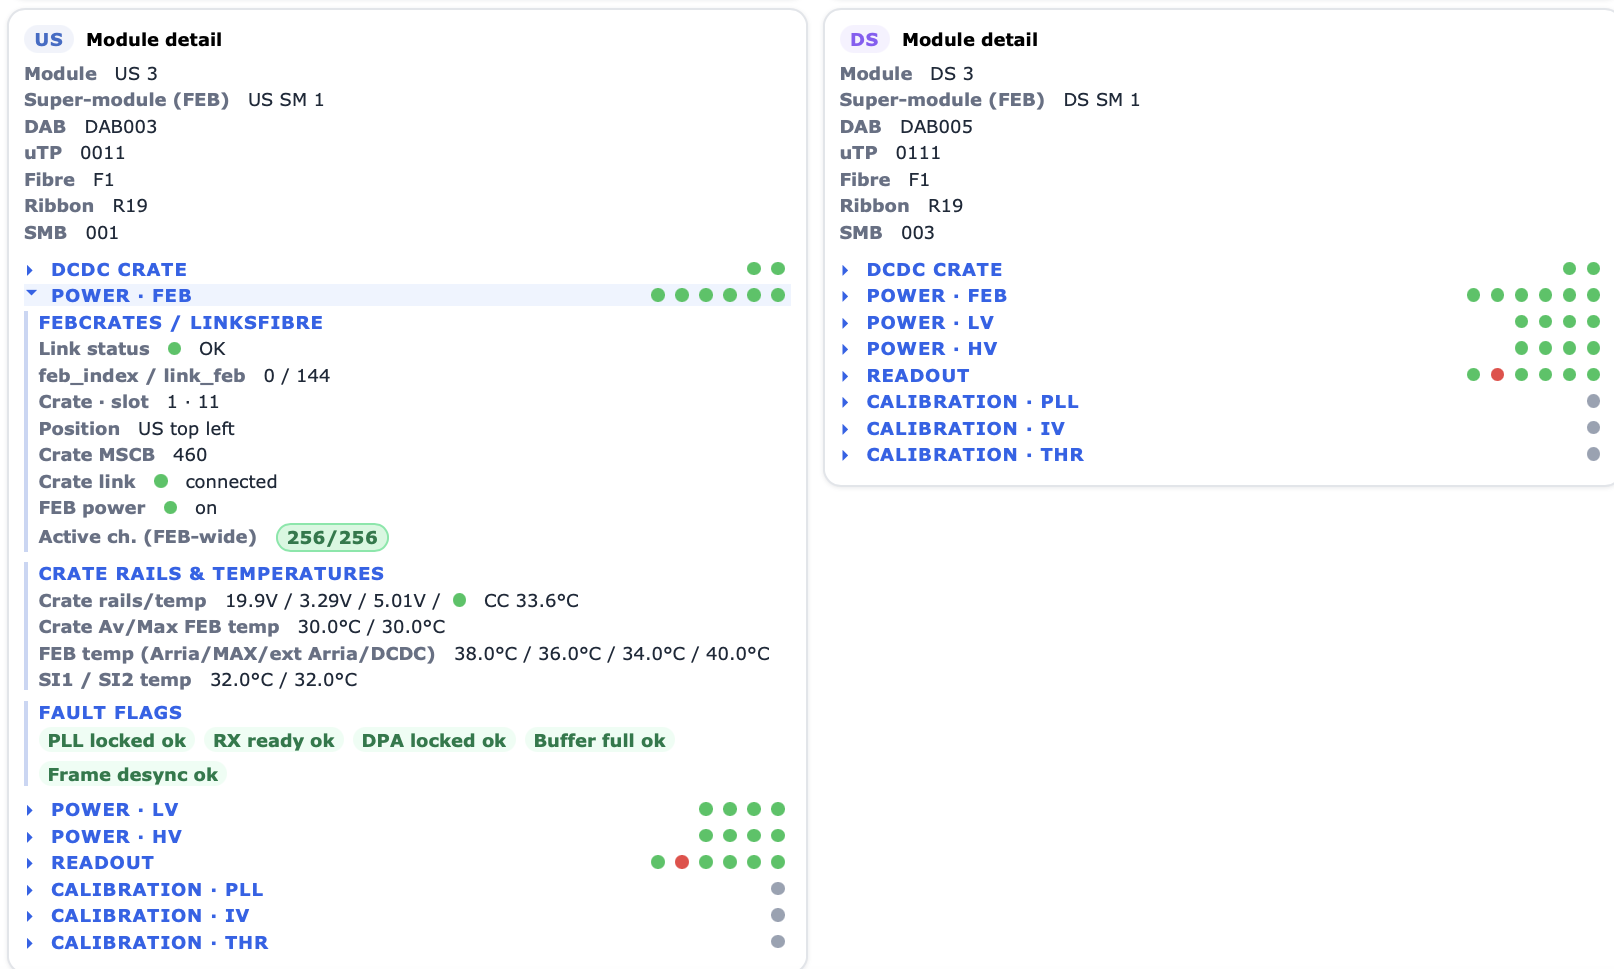
\includegraphics[height=5.3cm]{../imgs/img_geometry_drilldown.png}
      \end{center}
    \end{column}
  \end{columns}
\end{frame}

\begin{frame}{What's hardcoded vs.\ what's live}
  \begin{center}
  \renewcommand{\arraystretch}{1}
  \begin{tabular}{@{}c p{9cm}@{}}
    \tikz\node[rounded corners=2pt, inner sep=4pt, minimum width=2.4cm, fill=ETHGreen!12, draw=ETHGreen, thick, font=\small\bfseries, text=ETHGreen!55!black]{SAFE}; &
      Compile-time constants \\[4mm]
    \tikz\node[rounded corners=2pt, inner sep=4pt, minimum width=2.4cm, fill=ETHBlue!12, draw=ETHBlue, thick, font=\small\bfseries, text=ETHBlue!65!black]{SELF-HEALING}; &
      Name-pattern filters (\texttt{"SMB\_"}, \texttt{"SciFi CH"}) \\[4mm]
    \tikz\node[rounded corners=2pt, inner sep=4pt, minimum width=2.4cm, fill=ETHRed!12, draw=ETHRed, thick, font=\small\bfseries, text=ETHRed!55!black]{REAL RISK}; &
      Curated lists: \texttt{SciFi\_Programs.js} (7), \texttt{SciFi\_Alarms.js} (10), \texttt{HV\_BOARDS} (32-cell board$\leftrightarrow$module map) \\[4mm]
    \tikz\node[rounded corners=2pt, inner sep=4pt, minimum width=2.4cm, fill=ETHGray!12, draw=ETHGray, thick, font=\small\bfseries, text=ETHGray!55!black]{LIVE}; &
      Everything else \\
  \end{tabular}
  \end{center}
  \bigskip
  \texttt{HV\_BOARDS} is the single biggest hardcoded piece on the whole page -- flagged, not yet ported into Python/ODB.
\end{frame}

\begin{frame}{Calibration entry points -- a deliberate simplification}
  \texttt{thr\_run.py} / \texttt{vbr\_run.py} / \texttt{pll\_run.py} bypass SciFi's own \texttt{CalibrationFactory} (never wired to a real entry point) and instead:
  \begin{itemize}
    \item build \texttt{Detector} + \texttt{Calibration} \textbf{directly}
    \item open their \textbf{own} \texttt{MidasClient}, with \texttt{try/finally: disconnect()}
  \end{itemize}
  \bigskip
  \begin{block}{Judged safer than pixel's own pattern}
    Pixel passes PySequencer's \texttt{seq} object in as the client -- never independently verified. SciFi's explicit connect/disconnect is a stronger guarantee.
  \end{block}
\end{frame}

\begin{frame}{From design to a real save}
  \begin{block}{\texttt{.root} layout}
    5 trees -- \texttt{Meta}, \texttt{RawScan}, \texttt{Results}, \texttt{Conditions}, \texttt{ChannelMasks} -- the shape was restructured once per-module/per-ASIC parameters were properly pinned down.
  \end{block}
  \bigskip
  \texttt{ResultSaverROOT} (per-tree upsert by key), \texttt{ResultSaverCDB} (opt-in POST to \texttt{mu3edb0/detcal}), and a local cache of the most recent per-FEB calibration are implemented and wired, reconciled with a colleague's parallel branch.
\end{frame}

\begin{frame}{The SciFi detector, briefly}
  \begin{columns}[onlytextwidth,T]
    \begin{column}{0.42\textwidth}
      \footnotesize
      \begin{itemize}\setlength{\itemsep}{1pt}
        \item \textbf{2 rings}, US / DS -- 12 modules each; \textbf{24 SMB} (12+12) merge into 12 super-modules via a passive DAB.
        \item \textbf{12 FEB} (1:1 with LV); \textbf{96 ASIC} (32 ch.\ each) $=$ \textbf{\textcolor{pwrcolor}{3072 channels}}; \textbf{24 HV channels} (1:1 with SMB).
        \item Each module: \{side, ring position, readout end\} -- the same key used across \textbf{ODB}, \textbf{geometry}, and \textbf{calibration}.
        \item SMB and DAB connect via microtwisted-pair links, carrying the raw \textbf{MuTRiG3} data downstream.
      \end{itemize}
    \end{column}
    \begin{column}{0.55\textwidth}
      \begin{center}
      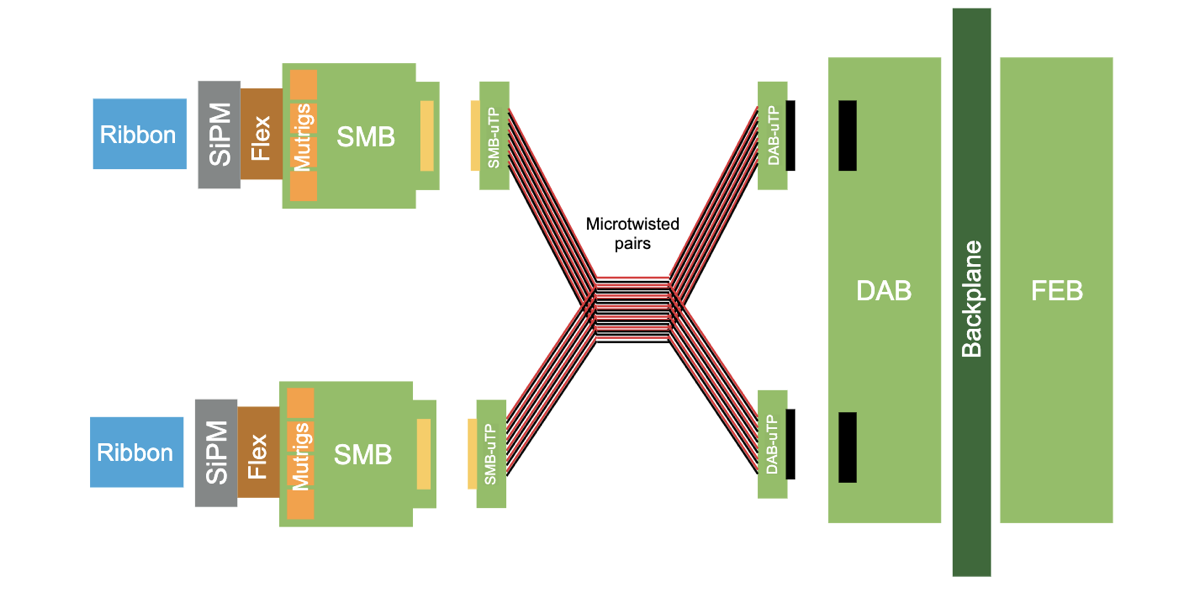
\includegraphics[width=\linewidth]{../imgs/img_signal_chain.png}
      \end{center}
    \end{column}
  \end{columns}
\end{frame}

\begin{frame}{Calibration: threshold scan}
  \vspace{-8mm}
  \begin{columns}[onlytextwidth,c]
    \begin{column}{0.47\textwidth}
      \small
      \begin{itemize}\setlength{\itemsep}{6pt}
        \item \textbf{\textcolor{calcolor}{ScanThr}} finds the right discrimination point on every channel.
        \item Walks the \textbf{threshold} up per channel, reading the rate curve to find the crossing points at 0.5, 1.5 and 2.5 p.e.
        \item Runs independently per \textbf{FEB} -- any subset of the detector can be (re-)calibrated on its own, and the result is what actually gets loaded as the operating threshold.
      \end{itemize}
    \end{column}
    \begin{column}{0.47\textwidth}
      \begin{center}
      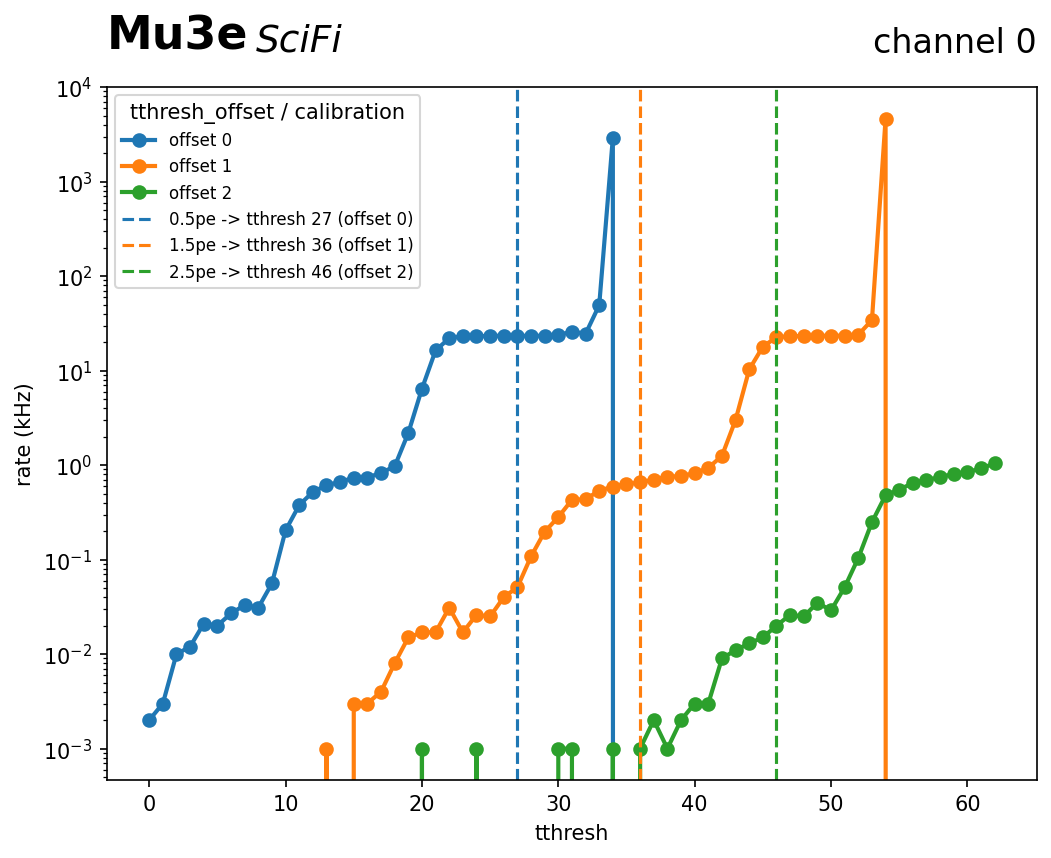
\includegraphics[width=\linewidth]{../imgs/img_scanthr_plot.png}
      \end{center}
    \end{column}
  \end{columns}
\end{frame}

\begin{frame}{Calibration: IV scan}
  \vspace{-8mm}
  \begin{columns}[onlytextwidth,c]
    \begin{column}{0.38\textwidth}
      \small
      \begin{itemize}\setlength{\itemsep}{6pt}
        \item \textbf{\textcolor{calcolor}{ScanVbr}} locates each SiPM's breakdown voltage.
        \item Takes the \textbf{derivative} of the IV curve and fits a \textbf{Gaussian} to its peak -- the fit mean $\mu$ gives $V_{br}$.
        \item Runs independently per \textbf{FEB} -- the result directly sets each SiPM's HV operating point (overvoltage), a real physics constant, not just a diagnostic.
      \end{itemize}
    \end{column}
    \begin{column}{0.58\textwidth}
      \begin{center}
      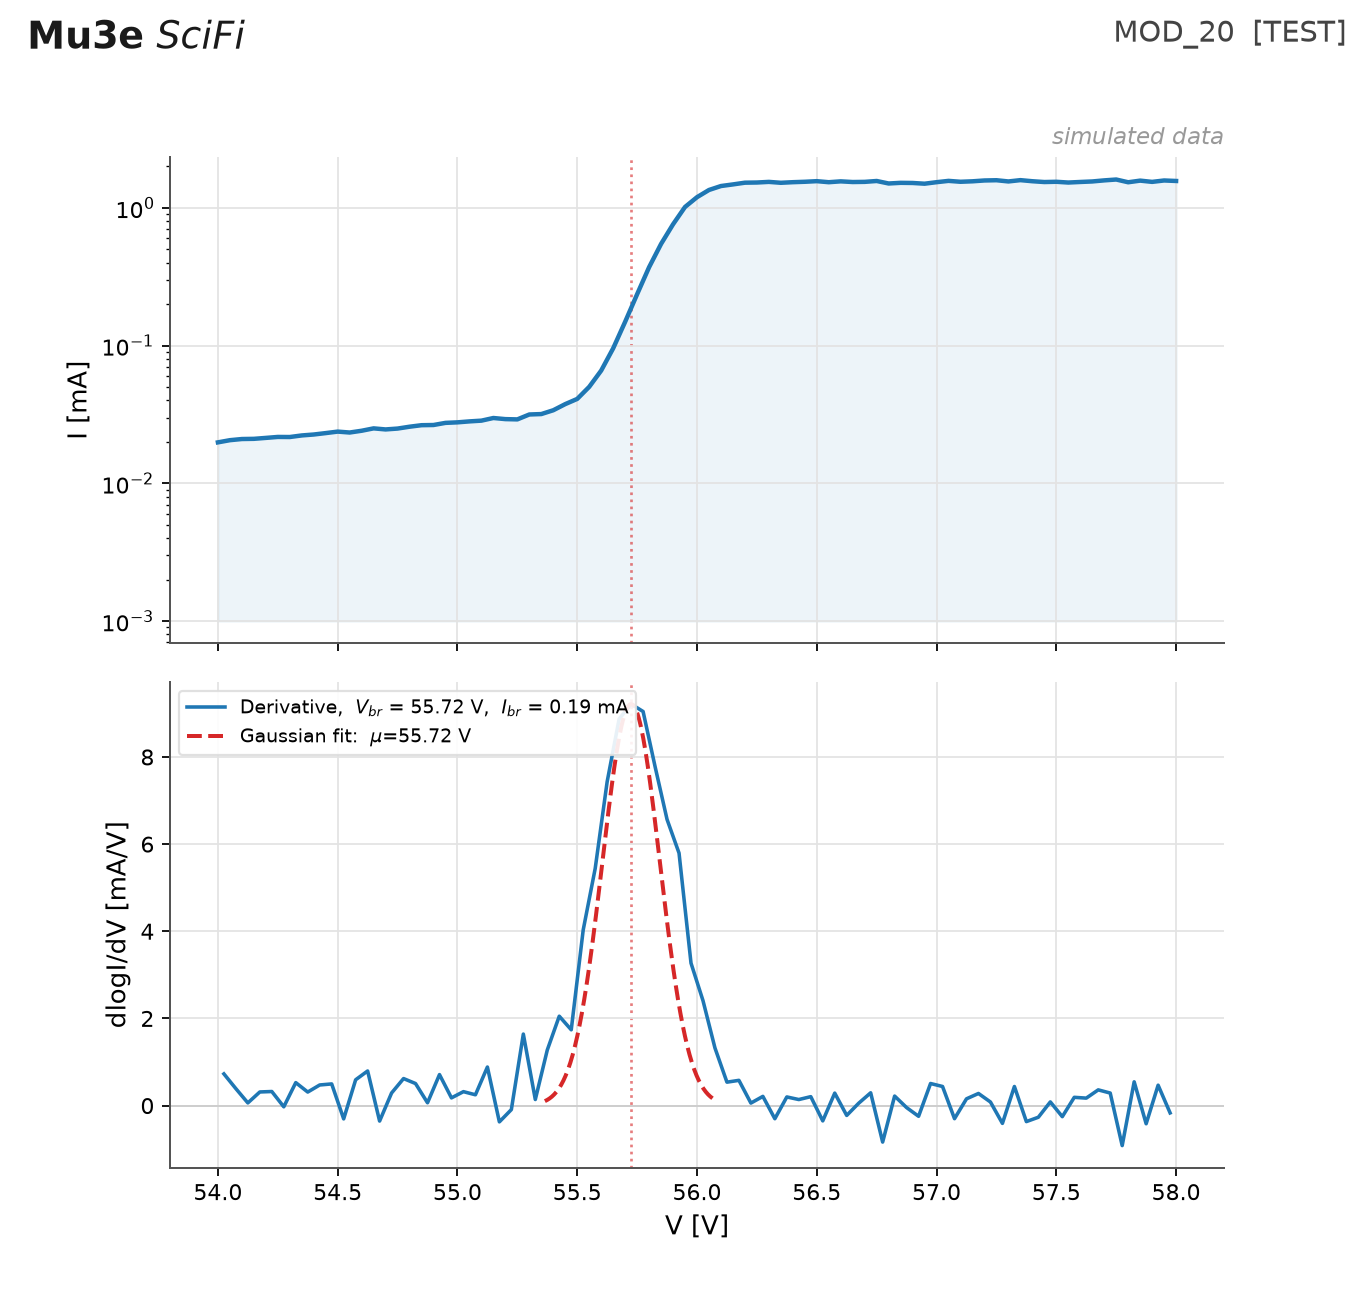
\includegraphics[height=7.0cm]{../imgs/test_plot_vbr.png}
      \end{center}
    \end{column}
  \end{columns}
\end{frame}

\begin{frame}{Configuration: PLL test}
  \vspace{-8mm}
  \begin{columns}[onlytextwidth,c]
    \begin{column}{0.4\textwidth}
      \small
      \begin{itemize}\setlength{\itemsep}{6pt}
        \item The \textbf{\textcolor{calcolor}{PLL test}} verifies every SMB recovers the clock from its data link.
        \item It histograms the recovered-clock \textbf{delay}: a genuinely \textbf{locked} PLL gives a \textbf{flat} distribution, an unlocked one a sharp peak.
        \item Pass/fail comes from the histogram \textbf{flatness} (mean vs.\ spread) -- one verdict per SMB.
      \end{itemize}
    \end{column}
    \begin{column}{0.58\textwidth}
      \begin{center}
      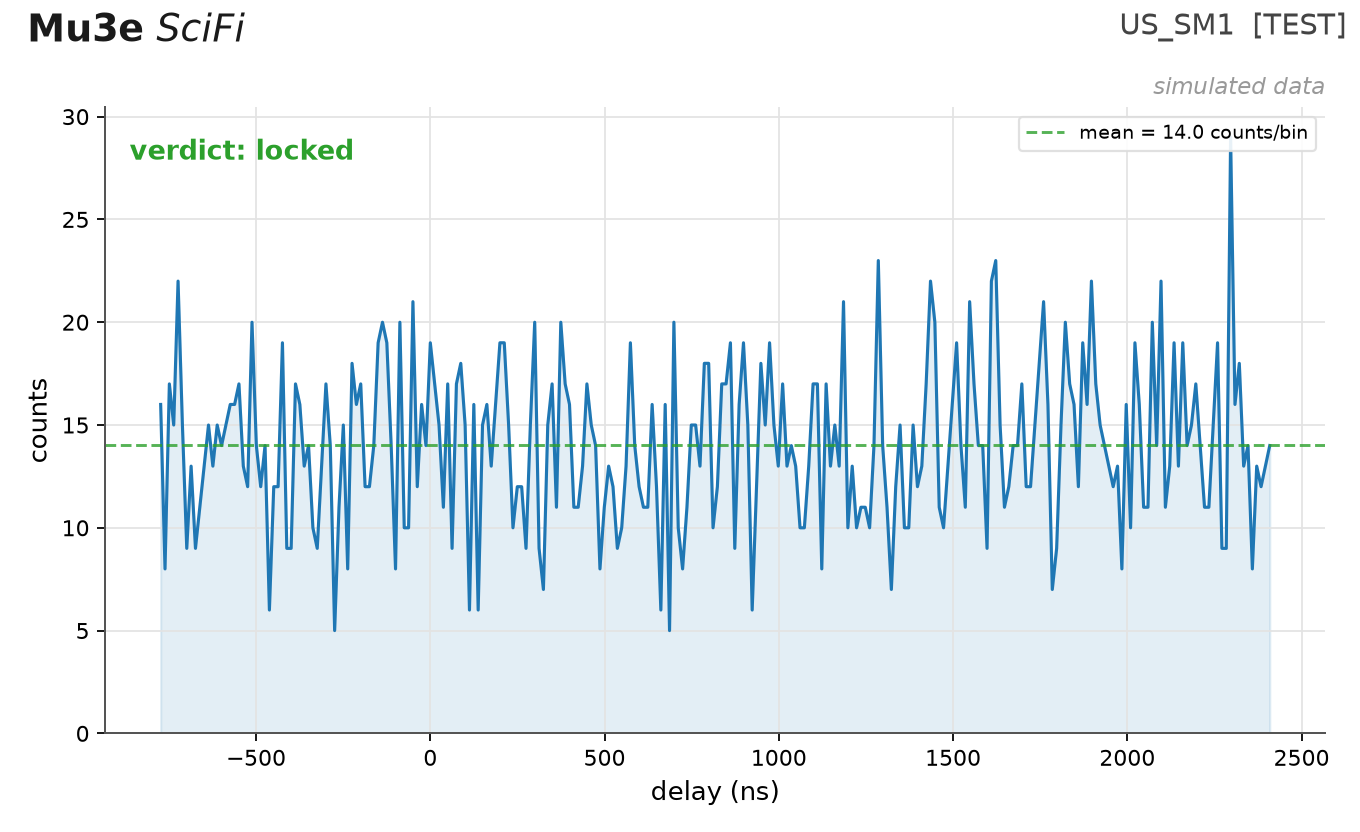
\includegraphics[width=\linewidth]{../imgs/test_plot_pll.png}
      \end{center}
    \end{column}
  \end{columns}
\end{frame}

\begin{frame}{What this leaves behind}
  \begin{itemize}\small\setlength{\itemsep}{1pt}
    \item \textbf{\textcolor{savecolor}{Result saving}} is fully implemented and wired -- the one piece that had to be ready for the data taking, and it is.
    \item The \textbf{shared code library} now properly covers SciFi, closing the gap with pixel: a real, reusable control and monitoring foundation, not a one-off.
    \item The \textbf{\textcolor{calcolor}{PLL verdict logic}} was corrected against real data -- a good example of the kind of mistake that only shows up once you actually run the thing.
    \item \textbf{\textcolor{confcolor}{Configuration}} grew into the detector's general hardware test hub, absorbing the old Readout tab entirely.
  \end{itemize}
  \smallskip
  \begin{center}
    \tikz\node[boxmeta, text=metacolor, minimum width=7.2cm, minimum height=0.8cm, font=\footnotesize]{Installed and working on \texttt{mu3ebe}: LV, HV, FEBs, Readout};
  \end{center}
  \smallskip
  \begin{center}
    \tikz\node[boxui, text=uicolor, minimum width=5.4cm, minimum height=0.8cm, font=\footnotesize]{What's still open};
  \end{center}
  \smallskip
  \small Everything is installed, wired, and ready. The one thing left is a full end-to-end workflow test, including a real calibration run, on \texttt{mu3ebe}.
\end{frame}

\begin{frame}{The detector, today}
  \vspace{4mm}
  \begin{center}
  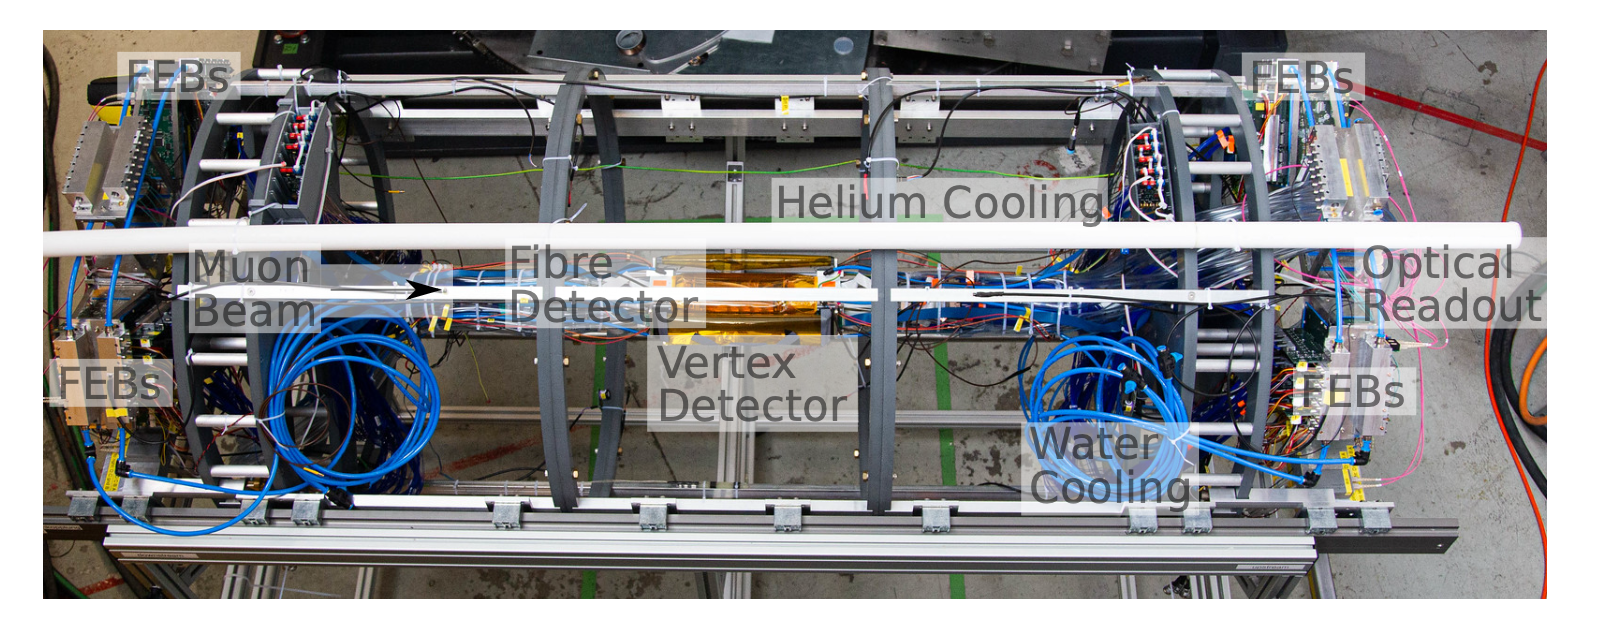
\includegraphics[width=0.98\linewidth]{../imgs/detector_prototype.png}
  \end{center}
\end{frame}

\begin{frame}{A SciFi ribbon}
  \begin{center}
  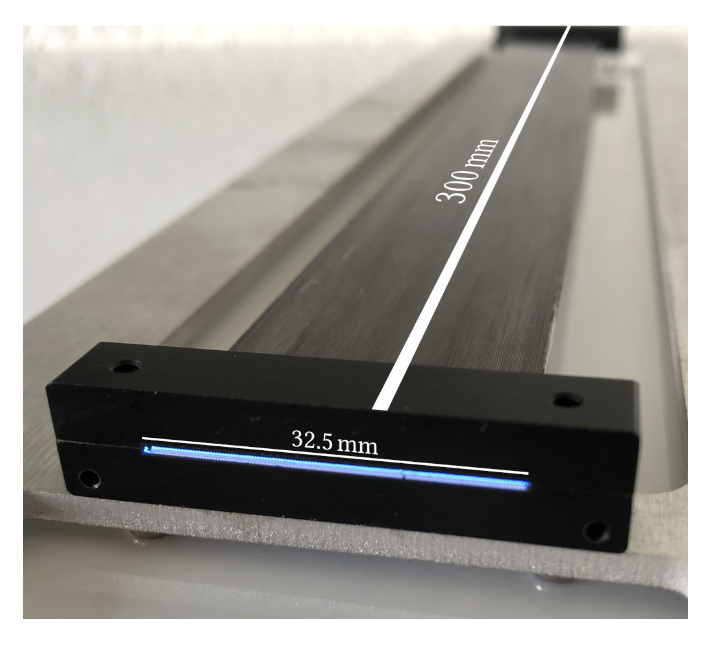
\includegraphics[height=6.8cm]{../imgs/fiber_picture.png}
  \end{center}
\end{frame}

\end{document}
